%Umberto Zarantonello 17-06-21

\section{Modello Standard}
La lagrangiana del modello standard è una formula che riassume in poche righe la descrizione attuale di tutte le interazioni.
\begin{equation}
L=-\frac{1}{4}F_{\mu\nu}F^{\mu\nu}+i\bar{\psi}\overline{D}\psi+\psi_i y_{ij}\psi_j\phi+|D_\mu\phi|^2+V(\phi)
\end{equation}

Innanzitutto si parla di lagrangiana, perché le interazioni in quella che è la fisica dei campi vengono descritte con quello che è il formalismo della meccanica analitica, questa non solo è una descrizione astratta della meccanica ma è anche il punto di partenza per le teorie quantistiche di campo.

Il primo termine della lagangiana è 
\begin{equation}
-\frac{1}{4}F_{\mu\nu}F^{\mu\nu}
\end{equation}
e rappresenta i campi dell'interazione.
In questo caso la forma è molto condensata, gli indici ripetuti rappresentano infatti una sommatoria su tutti i loro possibili valori.
In particolare con
\begin{equation}
F_{\mu \nu}=\partial_\mu A_\nu-\partial_\nu A_mu
\end{equation}
Dove $A_\mu$ è il potenziale dell'interazione.
Allo stato attuale non si è in grado di inserire la teoria della relatività generale all'interno di questa formula per cui le interazioni si limitano alle tre fondamentali: interazione elettromagnetica, interazione debole e interazione forte. 
Per esempio l'interazione coulombiana viene descritta da
\begin{equation}
A_\mu=(\Phi, \vec{A})
\end{equation}

Il secondo termine importante, che descrive le interazioni tra le particelle di materia e le particelle che trasmettono le forze è
\begin{equation}
i\bar{\psi}\overline{D}\psi
\end{equation} 
Anche in questo caso la rappresentazione è molto sintetica.
\begin{equation}
\overline{D}=\gamma^\mu D_\mu
\end{equation}
Rappresenta il prodotto delle matrici di Dirac per la derivata covariante (compatibile con la relatività speciale)
\begin{equation}
D_\mu=\partial_\mu +igA_\mu
\end{equation}
$A_\mu$ sono sempre i campi mentre, tornando al termine $\psi$ indica la funzione d'onda delle particelle di materia.
Questo tipo di derivata covariante esprime l'interazione.
La cosa straordinaria è che in queste teorie della meccanica quantistica relativistica, l'interazione si ottiene imponendo una condizione di simmetria (ovviamente compatibile con la relatività ) chiamata \emph{simmetria di Gauge}.
Questa simmetria prende il suo punto iniziale dall'analogia con l'elettromagnetismo estendendo però l'approccio a tutte le altre interazioni e i campi di interazione emergono in modo spontaneo imponendo questo tipo di simmetria.
La derivata covariante è proprio ciò che ci permette di ottenere le interazioni tra le particelle imponendo questa simmetria di Gauge.
$g$ è il parametro di accoppiamento di ogni tipo di interazione.

Gli ultimi tre termini
\begin{equation}
\begin{split}
&\psi_i y_{ij}\psi_j\phi\\
&|D_\mu\phi|^2+V(\phi)
\end{split}
\end{equation}
sono le interazioni con il campo di Higgs.
Perché la teoria sia relativisticamente invariante tutte le  particelle devono essere prive di massa, quindi sia i campi di materia che di interazione devono essere privi di massa.
Questo è imposto dalla teoria della relatività, una massa genererebbe una violazione di questa teoria.
In realtà si sa che sia le particelle di materia che alcune particelle di interazione hanno massa.
All'interno della teoria la massa si assume introducendo un campo scalare, \emph{il campo di Higgs}, che pervade tutto lo spazio e la massa avviene tramite una rottura spontanea di simmetria.
Questo tipo di interazione è quindi ciò che viene descritto da questi ultimi tre termini.

Questa lagrangiana è ciò che esprime quindi lo stato attuale della nostra conoscenza ed è estremamente bella ed elegante per la sua estrema sintesi.

%nuova sezione-----------------------------------------------------
\subsection{Modello standard della fisica delle particelle}
Questo modello è la sintesi di un centinaio di anni di studi sulla fisica delle particelle e delle interazioni fondamentali, non è quindi possibile attribuirvi né una data né un autore.

Siamo partiti dalla prima lezione vedendo che l'atomo è composto da nucleo ed elettroni, andando poi più in profondità si è visto che pure il nucleo è composto da protoni e neutroni.
Mentre in alcuni momenti si è pensato che il protone potesse essere una particella fondamentale, abbiamo visto che pure lui è composto di particelle più piccole.

Quali sono quindi le particelle fondamentali?
innanzitutto possiamo dire che per quanto ne sappiamo, l'elettrone è una particella fondamentale
\[
e^-
\]

Abbiamo visto poi che protoni e neutroni sono costituiti da quark
\[
p, n \longrightarrow d u
\]
in particolare il protone $p$ è costituito da due quark up $u$ e uno down $d$ mentre il neutrone $n$ da uno up $u$ e due down $d$.
Abbiamo visto anche che i quark hanno una carica frazionaria corrispondente a 
\[
\begin{split}
u\to +\frac{2}{3}e\\
d\to -\frac{1}{3}e
\end{split}
\]
Questa tra l'altro è una delle cose di cui non si ha ancora una teoria, è una conoscenza che si ha in quanto ci deve essere una logica e una connessione tra la carica e la composizione di protoni e neutroni ma non c'è ancora una teoria confermata che riesca a spiegare questo.

I quark non si sa se siano particelle fondamentali.

Ciò che si sa che per ragioni ignote, la natura ha deciso di replicare tutte le particelle che sono presenti nel protone e nel neutrone tre volte, ovvero esistono particelle instabili più  pesanti che replicano i quark ad energie più elevate.
Queste particelle in questo momento non esistono ma hanno contribuito alla creazione dell'universo nei suoi primi istanti di vita.

Il modello standard delle particelle fondamentali si basa sullo schema mostrato in figura.
\begin{figure}[h]
\centering
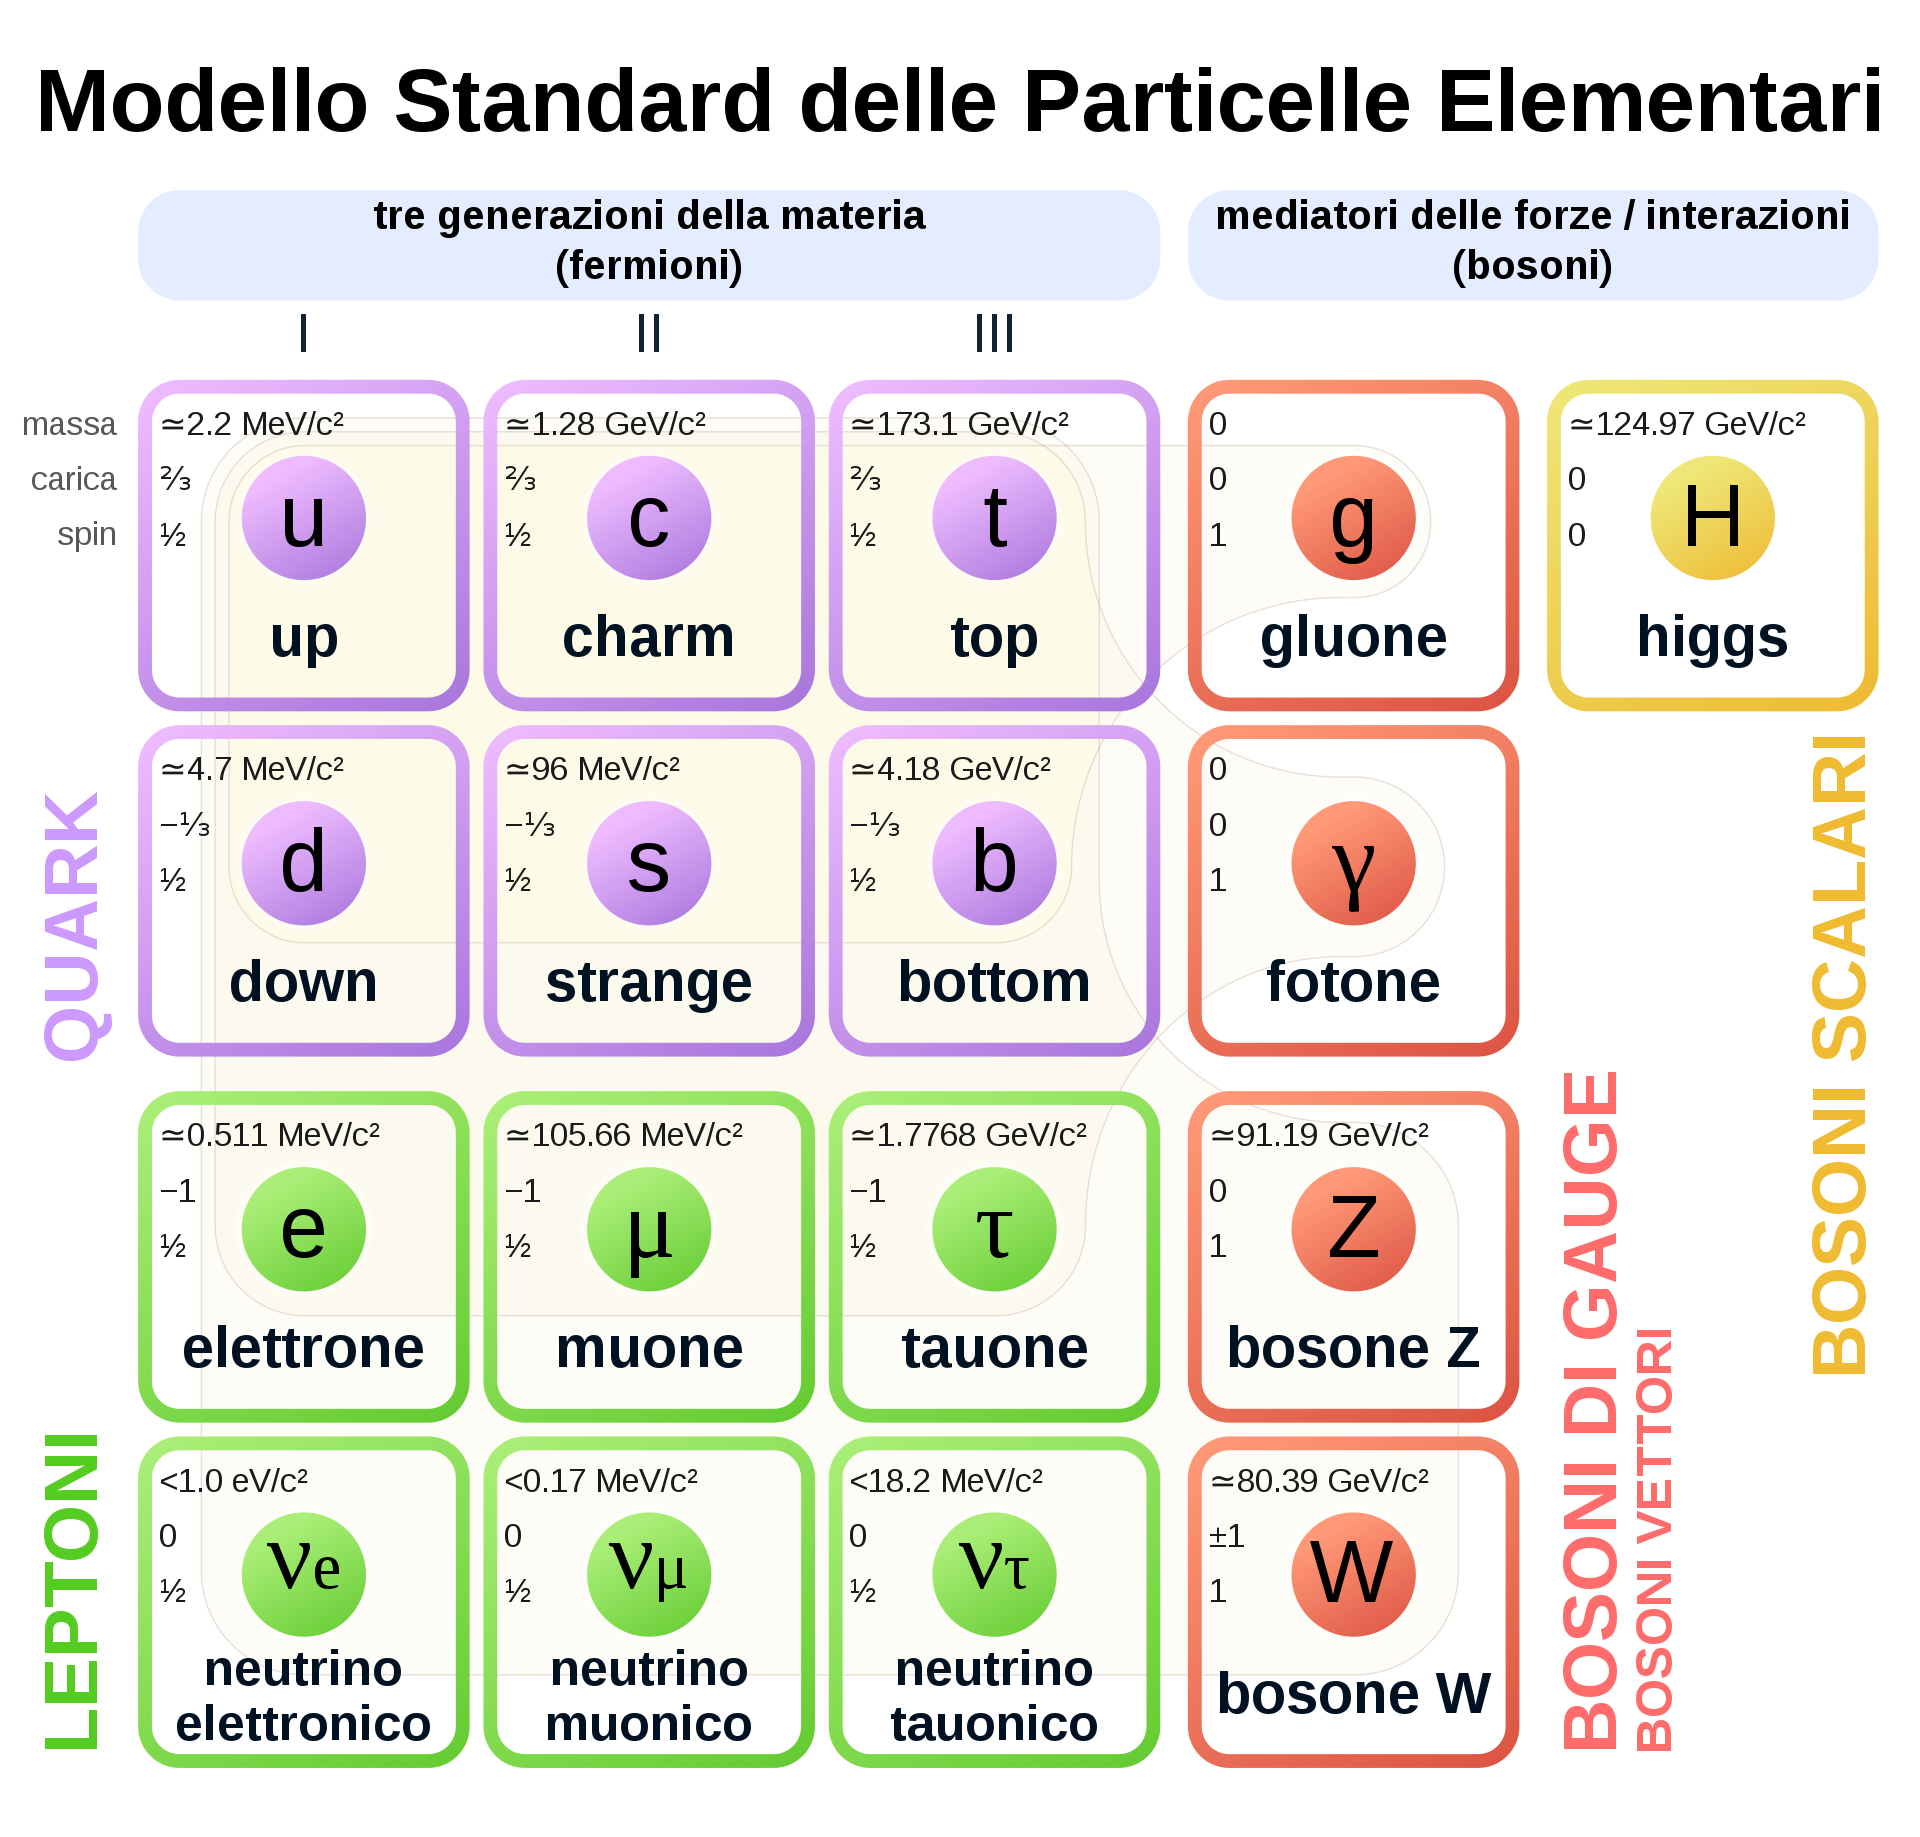
\includegraphics[width=180pt]{fig9_01}
\end{figure}

Come si può vedere i quark up e down sono sulla prima colonna, in alto sono indicate le masse.
Le particelle nella prima riga hanno carica pari a $2e/3$ mentre le particelle nella seconda riga $-1e/3$.
Le masse dei quark up e down sono ciò che definisce la massa di protone e neutrone, noi attribuiamo alla differenza tra le masse dei quark la causa della differenza di massa tra $p$ ed $n$ ma come si può vedere queste masse sono dell'ordine del $MeV$ quando invece le masse delle particelle nucleari sono dell'ordine del $GeV$.
Bisogna quindi attribuire gran parte della massa alle interazioni tra i quark (massa relativistica) ed è proprio per questo che non è possibile descrivere i quark all'interno del protone con le equazioni di Schroedinger, serve una teoria quantistica relativistica.

Al di sotto del quark down troviamo poi l'elettrone e il neutrino elettronico, rispettivamente di massa $0,5MeV$ e $~0eV$, ora in realtà si sa che il neutrino deve per forza avere massa, in quanto esistono delle condizioni in cui il neutrino può cambiare tipo e questo può avvenire solo nel caso che abbia massa.
Procedendo sulla stessa linea delle righe dei quark anche in questo caso, la riga dei neutrini ha carica $0$ e la riga dell'elettrone condivide carica $-1$.

Come già anticipato, la natura ha replicato queste particelle ma con un aumento di massa e il risultato di ciò sono le particelle che si trovano nelle due colonne successive.
Tutte le particelle che fanno parte delle prime tre colonne sono i fermioni, condividono lo spin $s=1/2$ e soddisfano la statistica di Fermi-Dirac, questi sono poi suddivisi in quark, posti nelle prime due righe, e leptoni, occupanti le ultime due righe.

Nell'ultima colonna sono posti i bosoni di Gauge che sono le particelle che al posto della statistica di Fermi Dirac rispettano la statistica di Bose Einstein.
Queste particelle sono i mediatori delle forze che regolano le particelle.
Sulla prima riga abbiamo il fotone $\gamma$ che è mediatore della forza elettromagnetica e che ha massa nulla.
Sotto sta il gluone $g$, mediatore della forza forte, anch'esso a massa nulla.
Mentre nelle ultime due righe abbiamo i mediatori della forza debole, ovvero il bosone $Z_0$ con una massa di $90GeV$ e i bosoni $W_\pm$ con una massa di $80GeV$.
La forza debole non è debole perché di bassa intensità ma è debole proprio perché è trasmessa da questi bosoni estremamente massivi che rendono proprio debole la forza.

Al grafico è poi aggiunto il \emph{bosone di Higgs} di cui è stata dimostrata l'esistenza pochi anni fa e che ha una peso pari a $125GeV$.
Si può notare poi come non sia presente nessuna particella legata alla forza di gravità, questo è infatti un punto debole del modello standard, non c'è ancora nessuna teoria che riesca ad inserire correttamente la gravità nella fisica delle particelle.

Di difficile comprensione è la logica che sta dietro alle strutture che si vengono a creare, non si ha ancora una spiegazione alla logica del modello e per dire Steven Haoking ha passato tutta la sua vita a cercare una spiegazione e una teoria che potesse unire tutto.
Non si riesce a capire per esempio come mai il quark $top$ una massa pari a quasi 50 volte quella degli altri quark. 
Altro limite notevole del modello standard è che non si riesca ancora a prevedere senza dati esterni le masse delle singole particelle, questo fa comprendere quanto sia ancora acerba la teoria, infatti se fosse completa dovrebbe poter prevedere senza ausili esterni le masse e le strutture che ci vengono a formare.

I fermioni e i bosoni sono differenziati principalmente dalla statistica a cui soddisfano, il che non è poco infatti se per dire gli elettroni non fossero fermioni non esisterebbe la chimica, o per lo meno non come la conosciamo noi.

Una differenza tra la forza forte e la forza elettromagnetica è che mentre i fotoni non possono interagire tra di loro, i gluoni sono in grado di farlo.
Ciò è essenziale in quanto se i fotoni interagissero tra di loro il modo stesso in cui vediamo sarebbe diverso infatti i fotoni arrivano al nostro occhio indisturbati ma se interagissero allora si avrebbe che il nostro occhio dovrebbe rivelare degli agglomerati di particelle.

\paragraph{Interazioni fondamentali}
I quark, che interagiscono con tutti i tipi di forze, sono tenuti insieme grazie alla forza forte che riesce a superare la forza elettromagnetica che tende ad allontanarli.
Per questo motivo la forza forte ha una logica completamente diversa da quella elettromagnetica, in particolare si ha che i quark non possono esistere come particelle libere ma solo in combinazioni che danno luogo agli \emph{Adroni} che possono essere di due tipi:
\begin{itemize}
\item \emph{Mesoni}, costituiti da coppie ($q, \bar{q}$)
\item \emph{Barioni}, formati ($q, q, q$)
\end{itemize}
Ovviamente, come per le altre particelle, anche i quark possiedono degli antiquark con le stesse caratteristiche ma di carica opposta.
L'asimmetria che c'è tra la quantità di materia e di antimateria è uno dei misteri ancora irrisolti della fisica, il diverso comportamento tra materia e antimateria previsto dal modello standard riesce a spiegare infatti solo in minima parte questa asimmetria (è di circa $8$ ordini di grandezza più piccolo di quello che servirebbe per spiegare totalmente la dominanza della materia).

\begin{figure}[h]
\centering
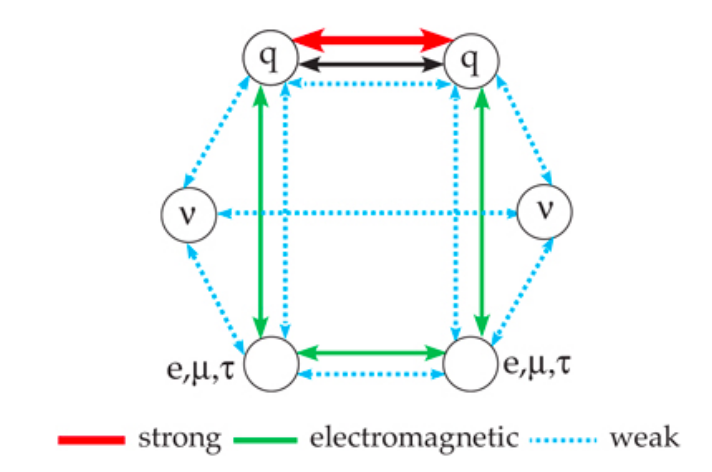
\includegraphics[width=180pt]{fig9_03}
\end{figure}
Per capire come interagiscono si consideri che ogni categoria di particelle (quark, leptoni e neutrini) ha la possibilità di interagire con le altre e con se stessa per mezzo di tre forze (forza forte, debole ed elettromagnetica).
I quark interagiscono tra di loro tramite la forza forte e sono le uniche particelle che interagiscono tramite questa forza.
Si ha poi che interagiscono tramite la forza elettromagnetica sia i quark tra di loro che i leptoni tra di loro e di conseguenza interagiscono anche i quark con i leptoni.
Infine per quanto riguarda la forza debole, i neutrini interagiscono sia con i quark che con i leptoni , i quark inoltre possono interagire sia coni leptoni che tra di loro, quindi l'unica interazione impossibile è dei leptoni con se stessi.

Le interazioni nel modello standard da un punto di vista formale si rappresentano con la lagrangiana del modello standard ma da un punto di vista più didattico ci viene ancora una volta in aiuto Feynman.
I diagrammi di Feynman non sono rappresentati nello spazio tempo ma rappresentano semplicemente un'interazione e volendoli figurare numericamente rappresenterebbero gli elementi di matrice caratterizzanti l'interazione.
\begin{figure}[h]
\centering
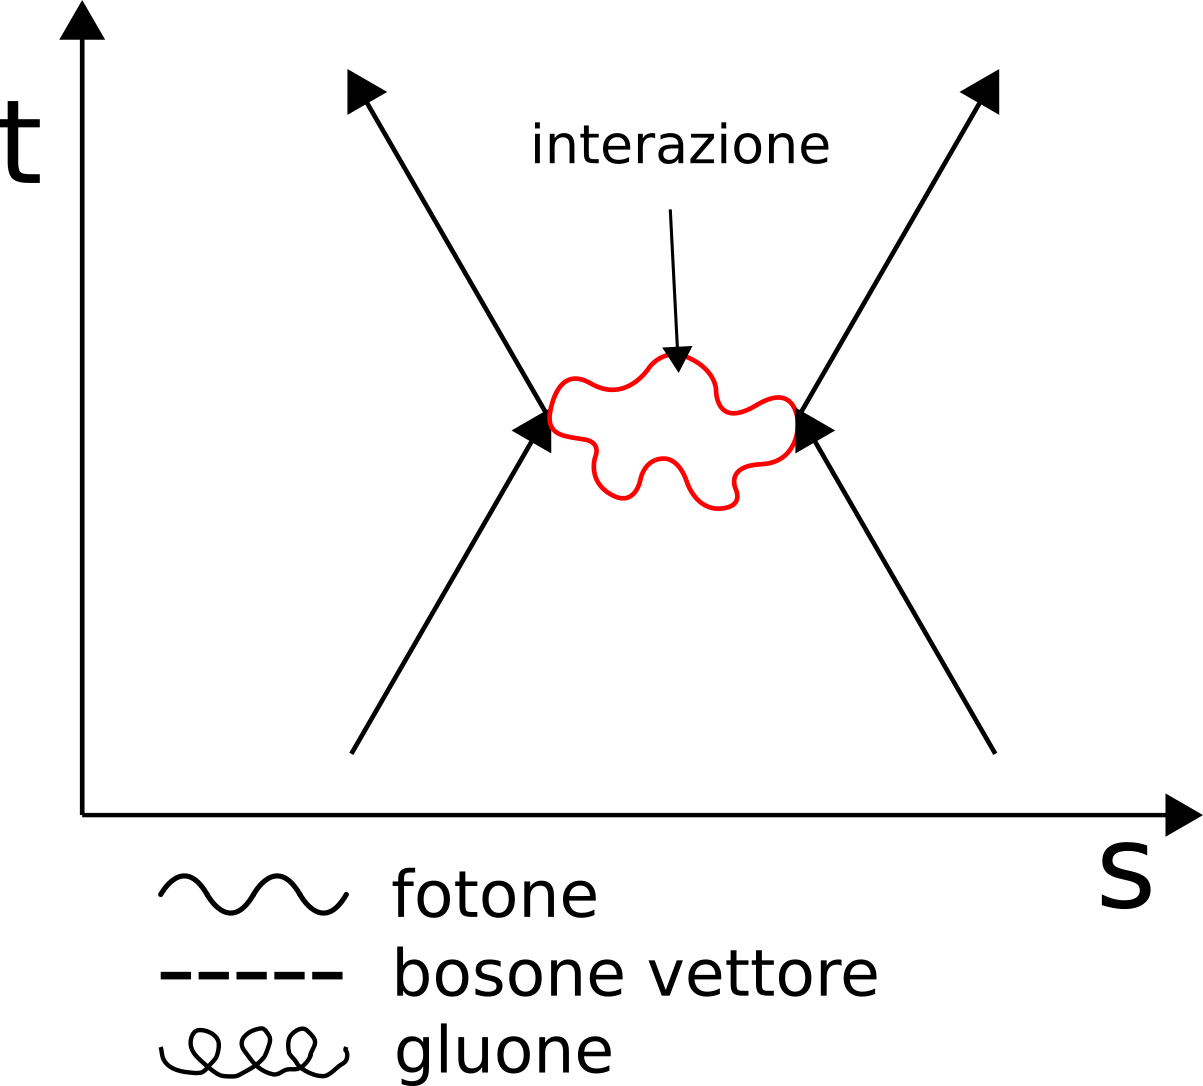
\includegraphics[width=180pt]{fig9_02}
\end{figure}

Le regole di base utilizzate per la rappresentazione di Feynman sono:
\begin{itemize}
\item Il tempo è solitamente fatto scorrere nella direzione verticale ma alle volte si può trovare pure nella direzione orizzontale.
Si predilige la verticalità ma non è una regola assoluta e bisogna intuirlo dal contesto.
\item Nella direzione orizzontale c'è lo spazio
\item Le particelle vengono rappresentate da dei vettori che si avvicinano, interagiscono e poi si allontanano.
Nel centro avviene l'interazione.
\item Le particelle che arrivano hanno una freccia che va in direzione del tempo nel caso siano particelle di materia ma se invece sono particelle di antimateria avranno una freccia nella direzione opposta al tempo.
\item Il tipo di interazione viene rappresentato dalla particella di scambio. 
Ci sono tre diverse simbologie:
\begin{itemize}
\item il fotone è rappresentato con una bisciolina;
\item il bosone vettore, mediatore della forza debole, corrisponde ad una linea tratteggiata;
\item Il gluone viene indicato con un'elica
\end{itemize}
\end{itemize}
Mentre nella rappresentazione classica le particelle interagivano tramite campi (secondo la descrizione di \emph{Faraday}, in meccanica quantistica le interazioni vengono appunto rappresentate da uno scambio di particelle.

\begin{figure}[h]
\centering
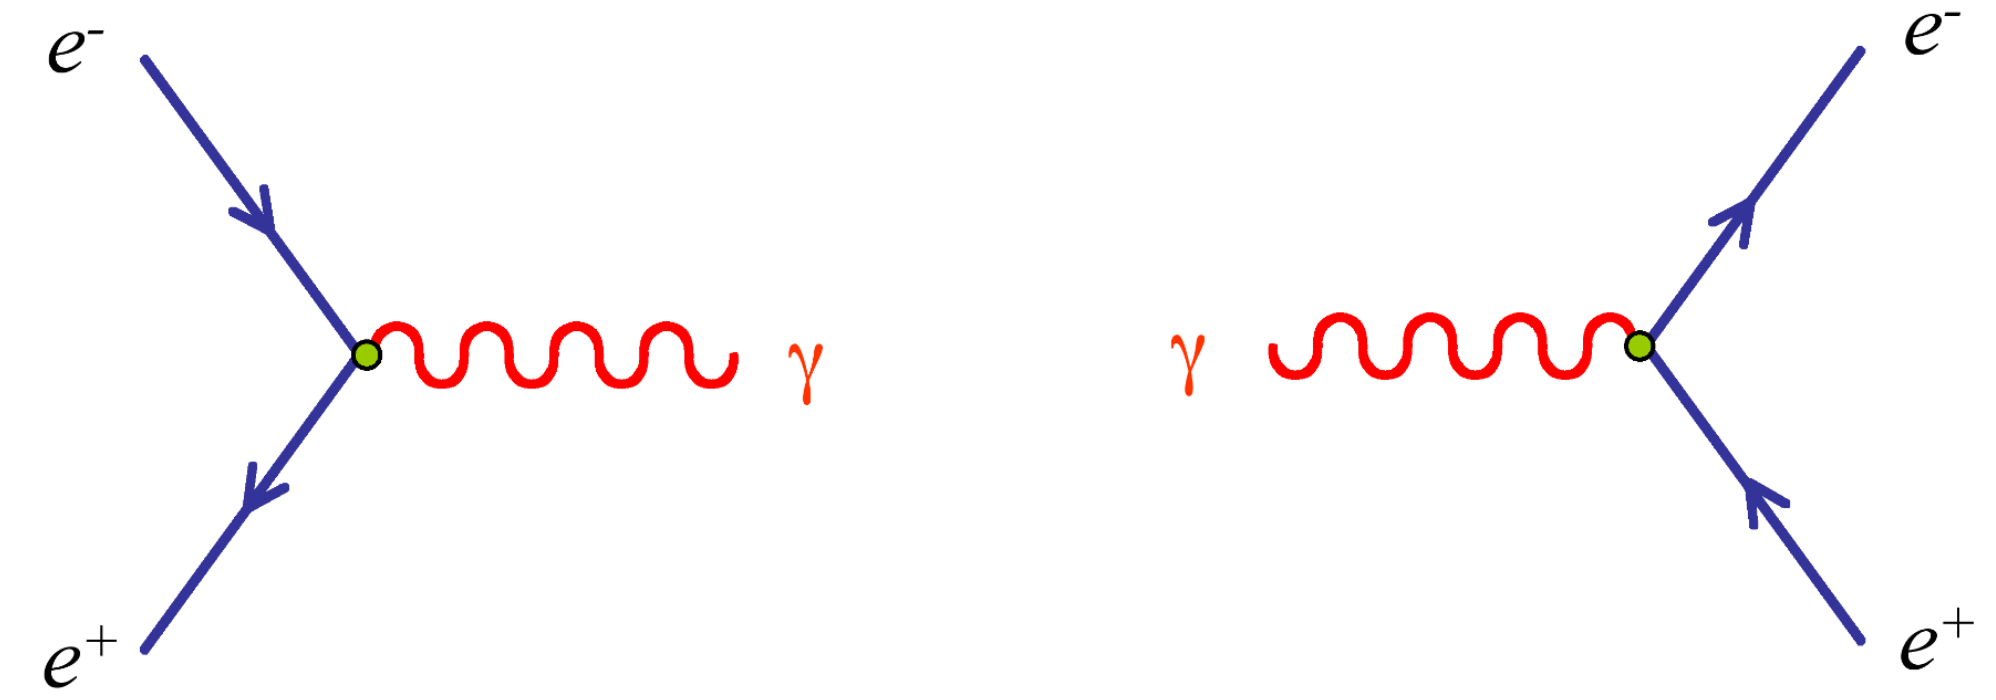
\includegraphics[width=220pt]{fig9_04}
\caption{Diagramma di Feynman della produzione di coppie e annichilimento}
\label{MD:9.04}
\end{figure}
Si consideri ora per esempio la produzione di coppie.
Il diagramma di Feynman dell'effetto è rappresentato nell'immagine ~\ref{MD:9.04}, considerando una linea temporale comune orizzontale, si ha da un lato la produzione di coppie e dall'altro l'annichilimento di una coppia.
Come si può notare il fotone come pure la particella e la sua antiparticella corrispondente  sono rappresentati secondo le regole di Feynman.

Ovviamente questi diagrammi devono soddisfare tutte le regole di conservazione della fisica.
\begin{itemize}
\item carica elettrica
\item numero barionico: se ho un protone prima dell'interazione dovrò avere un barione anche alla fine dell'interazione, per dire pure i quark possiedono un numero barionico
\[
q\to B=1/3 \hspace{1cm} \bar{q}\to b=-1/3
\]
\item numero leptonico: anche i leptoni devono essere creati in coppie leptone e antileptone
\[
e\hspace{0.2cm}L=1\hspace{1cm}\bar{\nu_e}=\hspace{0.2cm}L=-1
\]
fino ad ora c'era anche una legge sulla conservazione di flavor dei leptoni (tipologia di particella) ma dopo la scoperta delle oscillazioni dei neutrini questa legge è decaduta.
\end{itemize}

Facciamo ora un esempio.
Nel processo di decadimento del neutrone in protone abbiamo che il numero leptonico resta invariato ($L=0$) prima e dopo il decadimento, anche il numero barionico non necessita riequilibrio ($B=1$ prima e dopo l'evento) il numero di carica per rimanere invariato necessita si un bosone carico per questo l'interazione deve avvenire attraverso un bosone vettore $W^-$ di carica $-1$.
Il processo è già stato visto, per ricondurci alle particelle che conosciute bisogna vedere che poi il bosone vettore decade a sua volta generando un elettrone e un antineutrino elettronico.
Come si può notare anche in questo caso le regole di conservazione non vengono violate infatti $B=0$, $C=-1$ prima e dopo, mentre il numero leptonico $L=0$ prima dell'interazione e $L=1-1=0$ dopo.

Le particelle rappresentate dai vettori e poste solitamente ai lati dell'interazione sono quelle che vengono definite \emph{particelle reali}, mentre le particelle centrali, mediatrici dell'interazione, vengono definite \emph{particelle virtuali}.
Le particelle reali sono quelle che rispettano la regola alla base della relatività
\begin{equation}
E^2+p^2c^2=m^2c^4
\end{equation}
per le particelle virtuali invece questa legge non è necessaria, sono infatti particelle che esistono per un periodo di tempo limitato, legato al principio di indeterminazione di Heisemberg (se creo energia dal vuoto ma la faccio tornare nel vuoto in un tempo accettabile per il principio di indeterminazione allora lo posso fare).
Per indicare questo fenomeno si dice solitamente che le particelle virtuali non stanno sulla shell di massa (non soddisfano il principio di Einstien).
I fotoni possono quindi essere divisi in tre tipologie:
\begin{itemize}
\item per $E>pc$ \emph{Timelike}
\item per $E<pc$ \emph{Spacelike}
\item per $E=pc$ \emph{Lightlike}
\end{itemize}
I fotoni che rispettano le leggi di Einstein sono del tipo \emph{lightlike}.

Supponiamo che un elettrone emetta un fotone.
Supponiamo che il fotone sia a riposo, voglio far vedere che questo fotone deve essere per forza un fotone virtuale.
L'energia iniziale  del sistema è 
\begin{equation}
E_{in}=m_ec^2
\end{equation}
Se l'elettrone fosse in grado di emettere un fotone l'energia del sistema sarebbe
\begin{equation}
E_{fin}=m_ec^2+E_\gamma+\frac{p^2}{2m}
\end{equation}
Dove $E_\gamma$ è l'energia del fotone, mentre $p^2/2m$ è l'energia di rinculo.
Come si può vedere questa energia è maggiore di quella iniziale il che viola il principio di conservazione dell'energia.
Questo diventa possibile quindi solamente grazie al principio di indeterminazione di Eisenberg.
La stessa cosa succede per i mediatori della forza debole che, come abbiamo visto, hanno una massa di $70-80 GeV$.

Interagire, andando a considerare il significato basilare, vuol dire semplicemente avere una variazione della quantità di moto, quindi l'interazione con le particelle virtuali è un modo di rappresentare questo scambio di quantità di moto.
Grazie al principio di indeterminazione è possibile poi trovare il range della forza che dimostreremo essere dipendente dalla massa della particella scambiata.
Per rappresentare (figurativamente) questo tipo di schema supponiamo di avere due persone su due barche che si lanciano una palla.
\begin{figure}[h]
\centering
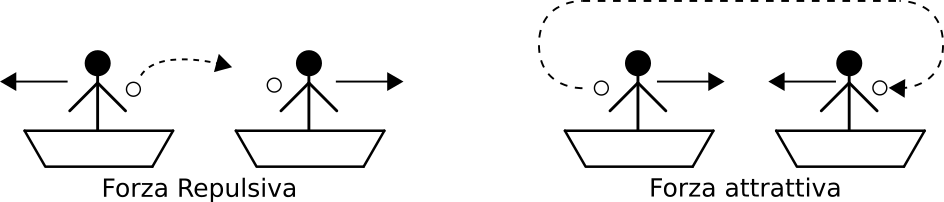
\includegraphics[width=250pt]{fig9_05}
\end{figure}

Come si può vedere nell'immagine a sinistra la palla che le due persone si scambiano è la rappresentazione della particella e il lancio della palla porta ad uno scambio di quantità di moto tra le barche che si allontaneranno.
La rappresentazione della forza attrattiva è un po' più complessa ma si può immaginare come il lancio di un boomerang da una barca all'altra che porterà dunque ad un moto inverso.
Ovviamente queste analogie sono solamente esplicative e no devono essere prese come una rappresentazione realistica del fenomeno.

Consideriamo ora l'interazione elettromagnetica, si approssimi $\hbar=c=1$.
Il principio di indeterminazione in questo caso afferma
\begin{equation}
Et\simeq \hbar=1
\end{equation}
Si vuole far vedere come l'interazione EM possa essere rappresentata con questo tipo di formulazione e comunque mantenere un range di interazione infinito della forza.
Supponendo $c=1$ si ottiene che 
\begin{equation}
E=p\hspace{0.5cm}t=r\hspace{0.2cm}\to\hspace{0.2cm}pr\sim 1\hspace{0.2cm}\to\hspace{0.2cm}p=\frac{1}{r}
\end{equation}
La forza diventa quindi la variazione della quantità di moto nel tempo
\begin{equation}
F=\frac{dp}{dt}=\frac{d}{dt}\left(\frac{1}{r}\right)=\frac{d}{dt}\left(\frac{1}{t}\right)=-\frac{1}{t^2}=-\frac{1}{r^2}
\end{equation}
Quindi siccome la massa del fotone $=0$ abbiamo che il range della forza elettromagnetica è infinito.
Si è arrivati a questa conclusione da un punto totalmente diverso rispetto alla dipendenza della legge di Coulomb come $1/r^2$.
In questo caso questo tipo di dipendenza deriva dal principio di indeterminazione di Eisenberg su una particella di massa nulla.

Il primo esempio di un'interazione mediata da una particella a massa non nulla deriva da un fisico giapponese chiamato Yukawa.
Si parte in questo caso dal fatto che si sa che la forza nucleare forte è limitata, il che vuol dire che il range della forza sarà limitato, vuol dire quindi che la particella dovrà avere massa diversa da zero.
Grazie a questa teoria Yukawa riuscì a predire l'esistenza del pione dimostrata successivamente.
Il punto di partenza della teoria è
\begin{equation}
E^2=p^2+m^2
\end{equation}
che esprime la relazione tra $E$ e $m$ della particella scambiata.
L'ipotesi è quindi che i nucleoni all'interno del nucleo si scambino una particella che deve essere per forza massiva per il fatto che abbiamo visto che il range è limitato.
Per passare all'equazione relativistica si applica il principio di corrispondenza
\begin{equation}
E\to i\frac{\partial}{\partial t}\hspace{1cm} p \to -i\bigtriangledown
\end{equation}
Possiamo quindi ora riscrivere la relazione energetica
\begin{equation}
-\frac{\partial^2}{\partial^2 t}\psi=-\bigtriangledown^2\psi+m^2\psi
\end{equation}
Questa è chiamata \emph{equazione di Klein-Gordon} ed è la prima equazione quantistica relativisticamente invariante, e descrive particelle con spin nullo ($s=0$).
Da notare che nel caso $m=0$ risolvendo l'equazione sopra nel caso stazionario si ottiene 
\begin{equation}
\bigtriangledown^2\psi=0 \to \psi=\frac{1}{r^2}
\end{equation}
Che corrisponde al caso visto prima per il campo elettrico.
Quello che interessa a noi ora rimane il caso per $m\not 0$
\begin{equation}
\bigtriangledown^2\psi =\frac{1}{r^2}\frac{d}{dr}\left(r^2 \frac{d\psi}{dr}\right)=m^2\psi
\end{equation}
La soluzione di questa equazione è del tipo
\begin{equation}
\psi(r)=\frac{g_s}{4\pi r}e^{-\frac{r}{R}}
\end{equation}
dove $R=1/m$. 
Nel caso quindi in cui la particella mediatrice abbia massa, alla componente del campo, simile al caso elettrostatico, viene aggiunto l'esponenziale indicato sopra che ha una forte dipendenza da $R$.
Ponendo quindi il raggio d'azione pari a 
\begin{equation}
R\sim \frac{1}{fm}
\end{equation}
si ottiene una massa di $m\simeq 200MeV$.

%nuova sezione------------------------------------------------------
\subsection{Interazione di Forza Forte}
\begin{figure}
\centering
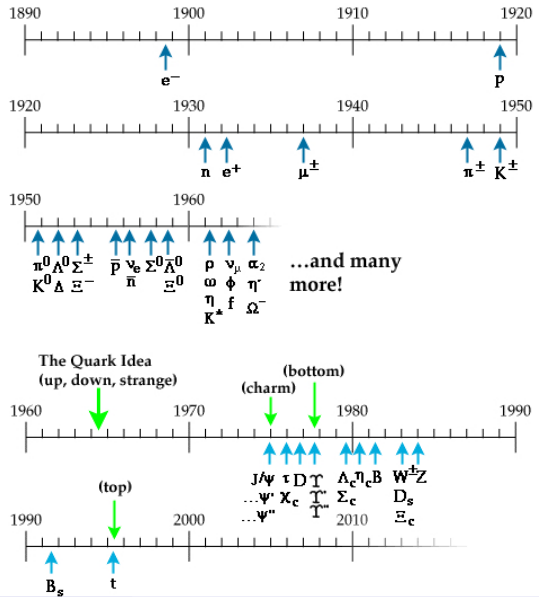
\includegraphics[width=280pt]{fig9_06}
\end{figure}

Da come si può vedere nel grafico la quantità di particelle scoperte dopo gli anni 50 e i nuovi investimenti sulla fisica nucleare è impressionante, bisogna considerare infatti che ai tempi si pesava di essere arrivati, ossia di aver trovato tutte le particelle che componevano il nucleo, tanto che la rivelazione del fatto che il pione di massa $200MeV$ non fosse il famoso mesotrone predetto da Yukawa aveva portato ad una serie di dubbi da parte delle eminenze fisiche del tempo.
Proverbiale fu quindi la teoria di Muray-Gellman che applicava le basi della teoria dei gruppi alla fisica subnucleare cercando di darne con un numero minimo di parametri una spiegazione completa, caso molto fortuito inoltre visto che quello che doveva essere un semplice espediente matematico si rivelò poi essere la realtà con la rivelazione successiva dei quark.
Queste particelle dopo essere state predette teoricamente furono rivelate e si ricominciò quindi a trovare una logica dietro tutte queste particelle.
Alla base della teoria sta la \emph{forza nucleare forte} che tiene legati i quark e provoca le interazioni che generano le varie particelle visibili nel grafico cronologico sopra.

\paragraph{Spettroscopia adronica}
La forza forte è una forza  che non distingue tra protone e neutrone.
Questa simmetria evidente che si genera tra protone e neutrone era stato spiegato inizialmente con quello che si chiama \emph{spin isotopico}.
Non è esattamente uno spin ma sfrutta la stessa matematica dello spin ovvero le matrici di Pauli.
In questo tipo di approccio l'obbiettivo è quello di rendere equivalenti protone e neutrone dal punto di vista dell'interazione forte, e quindi si vedeva il protone e il neutrone come doppietti di isospin a cui si assegnava spin $I=1/2$ al nucleone.
Per distinguere tra i due tipi di nucleoni si poteva sfruttare allora la stessa distinzione tra gli spin elettronici
\begin{itemize}
\item protone con spin up $I_3=+1/2$
\item neutrone con spin down $I_3=-1/2$
\end{itemize}
Questa è una nomenclatura che può essere utilizzata anche ai giorni nostri, in particolare nello spazio virtuale delle interazioni (con questo modello a spin) si possono rappresentare i nucleoni con due matrici
\begin{equation}
p=
\begin{pmatrix}
1\\0
\end{pmatrix}
\hspace{1cm}
n=
\begin{pmatrix}
0\\1
\end{pmatrix}
\end{equation}
Questo tipo di approccio, pur non essendo un approccio reale è molto utile da un punto di vista del calcolo.
In particolare seguendo questo modello si spin i pioni rappresentano degli stati di tripletto di questo spin.
\begin{equation}
\pi^+=
\begin{pmatrix}
1\\0\\0
\end{pmatrix}
\hspace{0.5cm}
\pi^0=
\begin{pmatrix}
0\\1\\0
\end{pmatrix}
\hspace{0.5cm}
\pi^-=
\begin{pmatrix}
0\\0\\1
\end{pmatrix}
\end{equation}
Questo era un primo modo per esprimere il fatto che l'interazione forte è indipendente dalla carica, bisogna considerare infatti che il concetto di quark non era ancora stato introdotto, si può comunque vedere che il concetto di base può essere applicato ed essere consistente anche con i quark
\begin{equation}
I(u)=I(d)=\frac{1}{2}\hspace{0.5cm} I_3(u)=+\frac{1}{2}\hspace{0.5cm}I_3(d)=-\frac{1}{2}\hspace{0.5cm}I(s)=I_3(s)=0
\end{equation}
dove $u, p, s$ indicano rispettivamente i quark \emph{up, down, s} e i valori $I_3$ indicano le proiezioni di spin nello spazio di isospin.
\'E utile conoscere questa terminologia perché il termine \emph{isospin} è utilizzato anche ai giorni nostri in quanto nell'interazione nucleare il fatto che non coinvolga alte energie non rende necessaria l'introduzione di quark più pesanti.

La particella scoperta successivamente (1947), trovata anch'essa nei raggi cosmici è il \emph{quark strano}.
Una delle peculiarità che si verificavano è che facendo collidere un $\pi^-$ (pione negativo) con un protone in una camera a nebbia si potevano vedere delle particelle che si collegavano a coppie.
\begin{equation}
\pi^-+p\longrightarrow K^0 \Lambda
\end{equation}
dove il prodotto è composto da $K^0$, un mesone, e una particella lambda $\Lambda$, i quali poi decadevano dando origine ad altre particelle
\begin{equation}
K^0\longrightarrow \pi^++\pi^-\hspace{1cm} \Lambda\longrightarrow\pi^-+p
\end{equation}
La peculiarità è che la sezione d'urto di produzione di questo tipo di reazione era una sezione d'urto pari a
\begin{equation}
\sigma\sim 1mb
\end{equation}
per un'energia di circa $1GeV$, il che corrisponde ai valori tipici dell'interazione forte, quindi queste particelle venivano prodotte per interazione forte.
La vita media di queste particelle corrispondeva invece a 
\begin{equation}
\tau_{K^0}\simeq 89ps
\end{equation}
Che per l'interazione forte è un tempo completamente fuori scala considerando che la forza forte ha tempi caratteristici di $10^{-22}, 10^{-23}s$ per cui queste particelle decadevano lentamente, con un tempo tipico dell'interazione debole, ed è per questo che sono state chiamate particelle strane.
Per questa ragione storica questa caratterizzazione delle particelle è stata definita come stranezza e sono stati attribuiti i valori 
\begin{itemize}
\item $K^0$ stranezza $=+1$
\item $\lambda$ stranezza $=-1$ 
\item $\pi, p$ stranezza $=0$
\end{itemize}
Per questo motivo storico di attribuzione di stranezza $+1$ a $K^0$ che poi $\Lambda$ quando è stata rinominata come quark $s$ è stata attribuita stranezza 
\begin{equation}
S(s)=-1
\end{equation}
mentre al suo antiquark
\begin{equation}
S(\bar{s})=+1
\end{equation}
Si potrà vedere poi che il mesone $K^0$ è costituito da un quark $\bar{d}$ e un quark $s$.

\paragraph{La teoria dei quark}
A metà degli anni $'60$ si arrivò finalmente all'introduzione del modello a quark di Gell-man, che riesce a spiegare tutte le particelle con un numero minimo di parametri, costituiti dai quark noti $u, d, s$.
La trattazione incredibilmente avvenne in modo indipendente da quella che è la teoria di \emph{deep inelastic scattering}, questo infatti ha spiegato la formazione interna del protone mentre la teoria di Gell-man puntava a spiegare le proprietà esteriori delle particelle (come lo spin e la carica).
Per creare questa teoria viene fatta quindi un'interpretazione del comportamento delle particelle.
I tre quark in pratica avrebbero dovuto spiegare la massa, la carica e lo spin, quindi almeno una di queste particelle doveva avere spin e carica (che poi nella teoria verrà attribuita a tutte le particelle come carica e spin frazionari).

Per esempio consideriamo due quark up $u$ con spin up e un quark down $d$con spin down, quella che si ottiene combinandoli è una particella con carica $C=+1$ e spin $s=1/2$, si è trovato quindi il protone $p$;
\begin{equation}
u\uparrow u\uparrow d\downarrow\hspace{1cm}C=+1\hspace{0.5cm}J=\frac{1}{2}\hspace{0.5cm}\to \hspace{0.5cm}p
\end{equation}
se ora prendiamo però le stesse particelle ma con tutte e tre spin solidale up quella che si trova è una particella con carica sempre pari a $C=+1$ ma spin $s=+3/2$ chiamata $\Delta^+$ e definita anche come risonanza del protone.
\begin{equation}
u\uparrow u\uparrow d\uparrow\hspace{1cm}C=+1\hspace{0.5cm}J=\frac{3}{2}\hspace{0.5cm}\to \hspace{0.5cm}\Delta^{+}
\end{equation}
La particella poi composta da tre quark up con spin up si ottiene la particella $\Delta^{++}$.
\begin{equation}
u\uparrow u\uparrow u\uparrow\hspace{1cm}C=+2\hspace{0.5cm}J=\frac{3}{2}\hspace{0.5cm}\to \hspace{0.5cm}\Delta^{++}
\end{equation}
Similmente si possono combinare tre quark down
\begin{equation}
d\downarrow d\downarrow d\downarrow\hspace{1cm}C=-1\hspace{0.5cm}J=\frac{3}{2}\hspace{0.5cm}\to \hspace{0.5cm}\Delta^{-}
\end{equation}
oppure introdurre il quark strange
\begin{equation}
s\downarrow s\downarrow s\downarrow\hspace{1cm}C=-1\hspace{0.5cm}J=\frac{3}{2}\hspace{0.5cm}\to \hspace{0.5cm}\Omega^{-}
\end{equation}

La combinazione dei quark non è casuale ma segue la stessa logica quantistica della combinazione di spin, il che vuol dire che volendo combinare due particelle con spin $1/2$ da luogo ad una combinazione di tripletto, in cui le particelle abbiano spin $1$ ma proiezione $1, 0, -1$ sull'asse $z$, più una combinazione di singoletto, in cui le particelle abbiano spin totale uguale a $0$
\begin{equation}
\begin{pmatrix}
\uparrow\\\downarrow
\end{pmatrix}
\otimes
\begin{pmatrix}
\uparrow\\\downarrow
\end{pmatrix}
=
\begin{pmatrix}
\uparrow\uparrow\\
\uparrow\downarrow+\uparrow\downarrow\\
\downarrow\downarrow
\end{pmatrix}
\oplus
\begin{pmatrix}
\uparrow\downarrow&\uparrow\downarrow
\end{pmatrix}
\end{equation}
Dobbiamo quindi immaginare una cosa simile per i quark ma con al posto del tripletto un ottetto.
\begin{equation}
\begin{pmatrix}
u&\\
d&s
\end{pmatrix}
\otimes
\begin{pmatrix}
u&\\
d&s
\end{pmatrix}
=
8\oplus 1
\end{equation}
Che in termini di teoria dei gruppi si scrive anche come
\begin{equation}
3 \otimes 3= 8 \oplus 1
\end{equation}
In termini tecnici si dice che $u, d, s$ sono una base della rappresentazione fondamentale del gruppo $SU(3) $ di simmetria di flavour.
In altre parole, i quark sono particelle quantistiche che quindi si combinano secondo le leggi della meccanica quantistica.
In meccanica quantistica la combinazione di particelle di spin $1/2$ si da luogo alla condizione di tripletto e di singoletto e allo stesso modo con i quark la combinazione da luogo alle condizioni di ottetto e singoletto.

Da notare che fino ad ora abbiamo considerato solamente lo spin per cui abbiamo tralasciato la possibilità che le particelle avessero momento angolare $L=0$ ma una complicazione ulteriore che genera ulteriori possibilità è proprio quella che i quark possiedano pure il momento angolare, cosa che in realtà accade.

Tutte le particelle composte da quark o antiquark vengono definiti \emph{adroni}, questi poi si dividono in \emph{barioni}, composti solamente da quark e in \emph{mesoni} composti da un quark e un antiquark.
\begin{figure}[h]
\centering
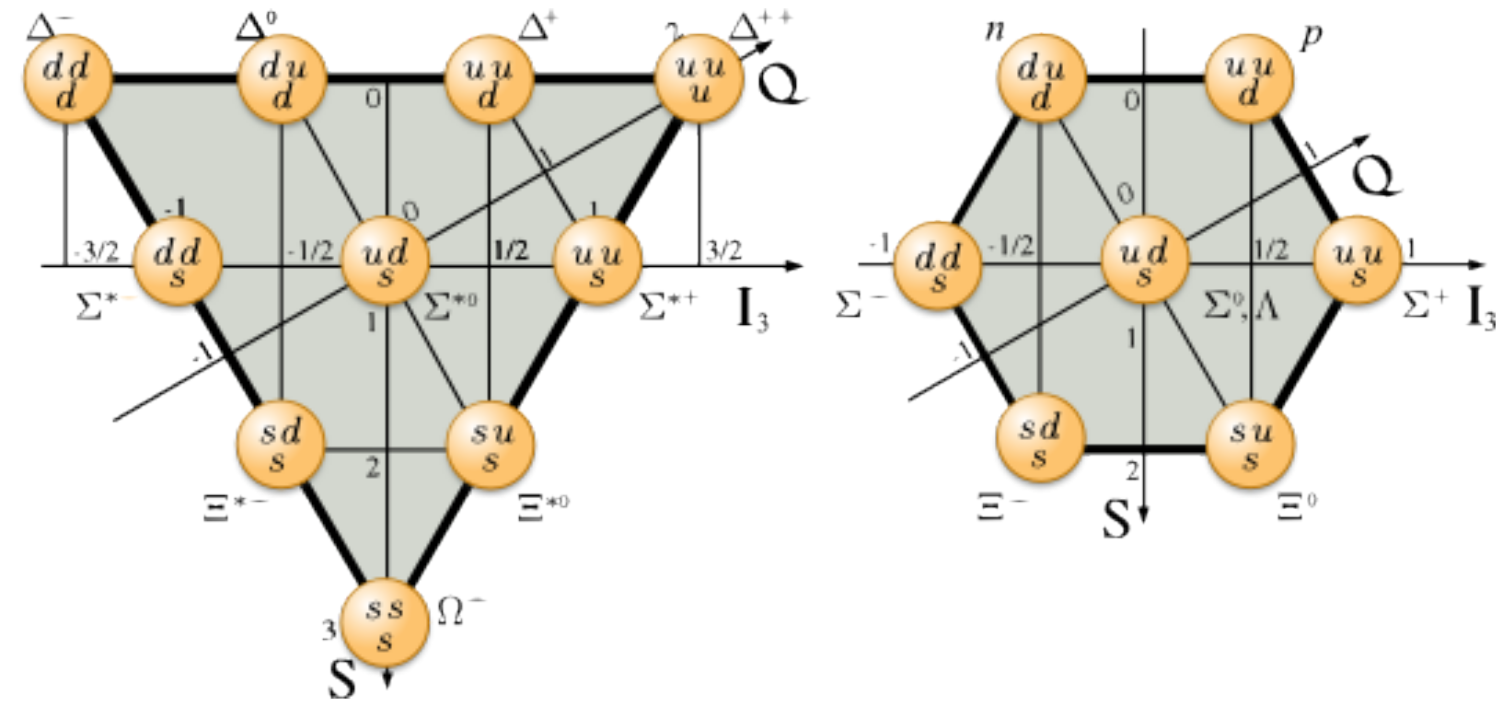
\includegraphics[width=250pt]{fig9_07}
\end{figure}

In figura sono mostrati i grafici che Gell-man creò per la classificazione delle particelle in base alle combinatorie di quark.
Come si può vedere la le figure sono piane e regolate da tre assi che ne definiscono le proprietà.
L'asse orizzontale indica il valore di isospin, l'asse verticale indica il valore della stranezza, l'asse obliquo indica la carica della particelle.
Ogni vertice rappresenta una particella differente.
Il grafico a destra indica il caso in cui lo spin totale sia $J=1/2$ mentre il grafico a sinistra indica il caso di spin totale $J=3/2$, quest'ultimo inoltre rappresenta il caso dell'ottetto inoltre rappresenta il caso visto prima dello stato di ottetto più singoletto infatti le particelle create sono esattamente nove.
Cosa particolare delle teorie fisiche è che per essere accettate devono avere anche un carattere predittivo che in questo caso viene dato dal fatto che la particella $\Omega^-$ fu predetta proprio da Gell-man e successivamente venne rivelata.

Si può ampliare la trattazione aggiungendo un asse che indichi il charm delle particelle portando così i grafici su un livello spaziale.
I grafici così generati sono posti sotto e definiscono quelli che vengono chiamati gli adroni charmati.
\begin{figure}[h]
\centering
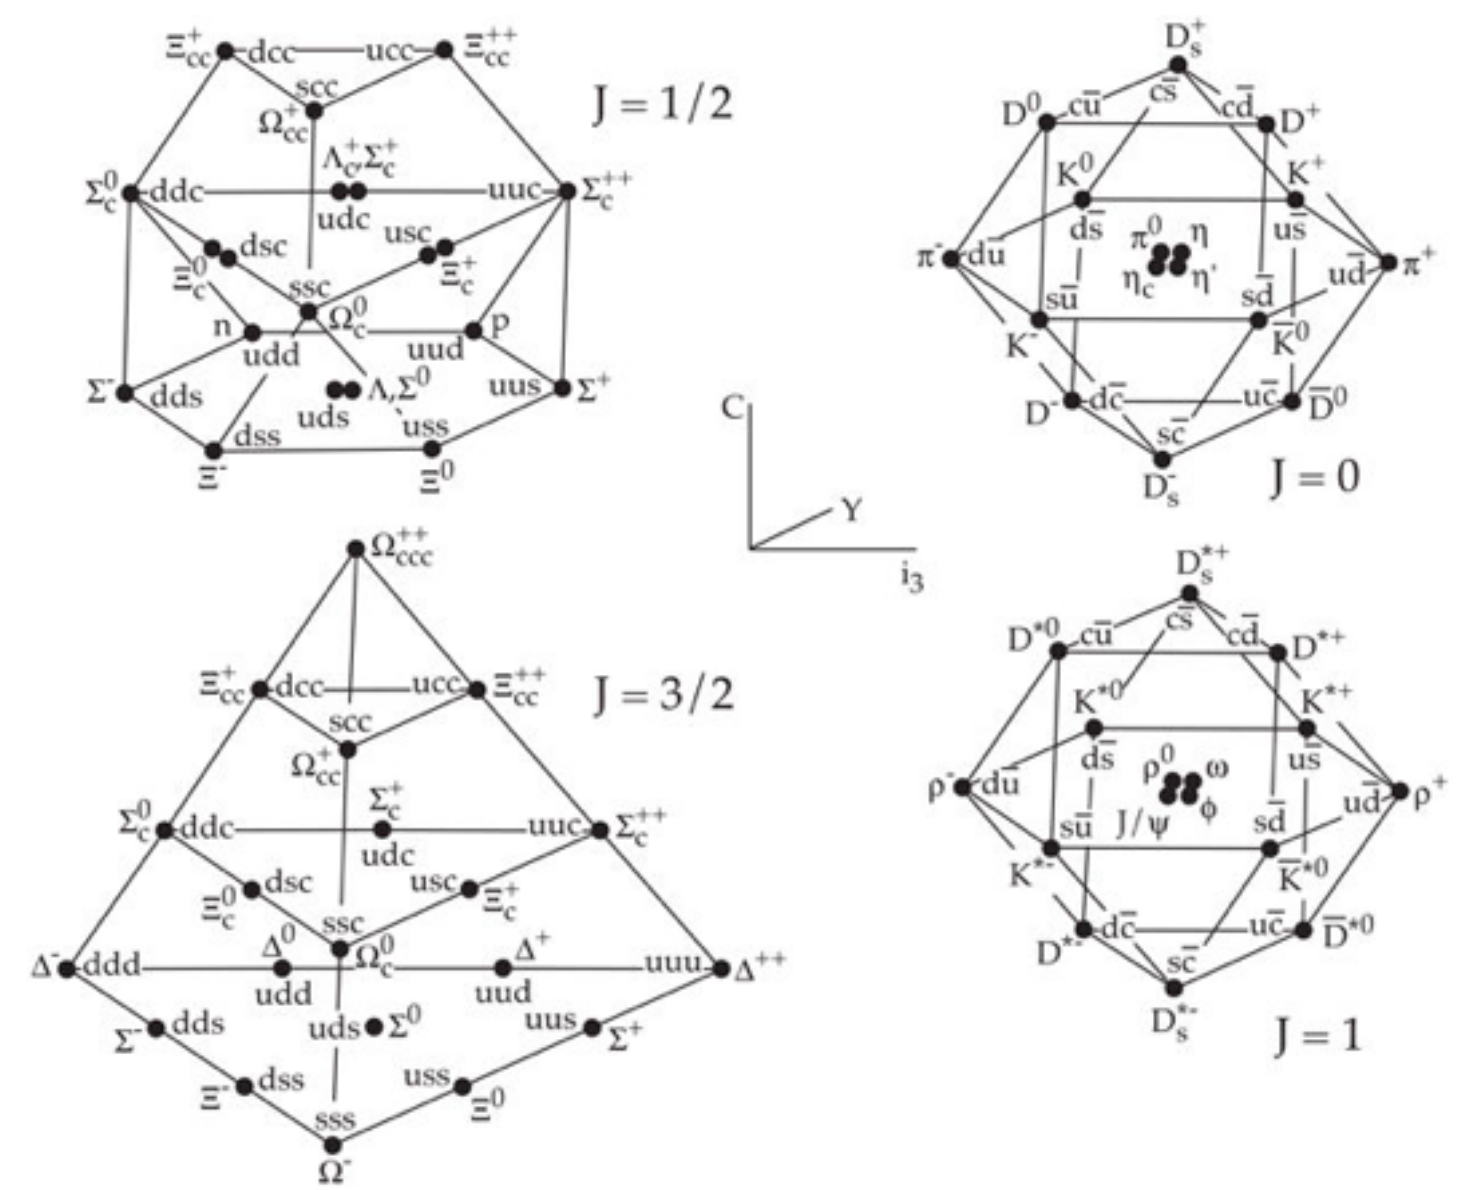
\includegraphics[width=250pt]{fig9_08}
\end{figure}

Volendo aggiungere trattazione, con l'aumento delle energie raggiunte dagli acceleratori si scoprì poi il quark bottom ancora più pesante del quark charm che ha generato altre particelle e quindi altri grafici.

Con la stessa logica sono stati poi studiati i \emph{mesoni}, che si differenziano dai barioni in quanto più piccoli poiché invece che essere generati da tre quark $qqq$ sono composti da un quark e un antiquark $q\bar{q}$.
Anche in questo caso le particelle possono essere raggruppate in funzione dello spin quindi in base al fatto che sia allineato, in questo caso si chiamano mesoni vettori, o antiallineato, chiamati mesoni (pseudo-)scalari.
\begin{figure}[h]
\centering
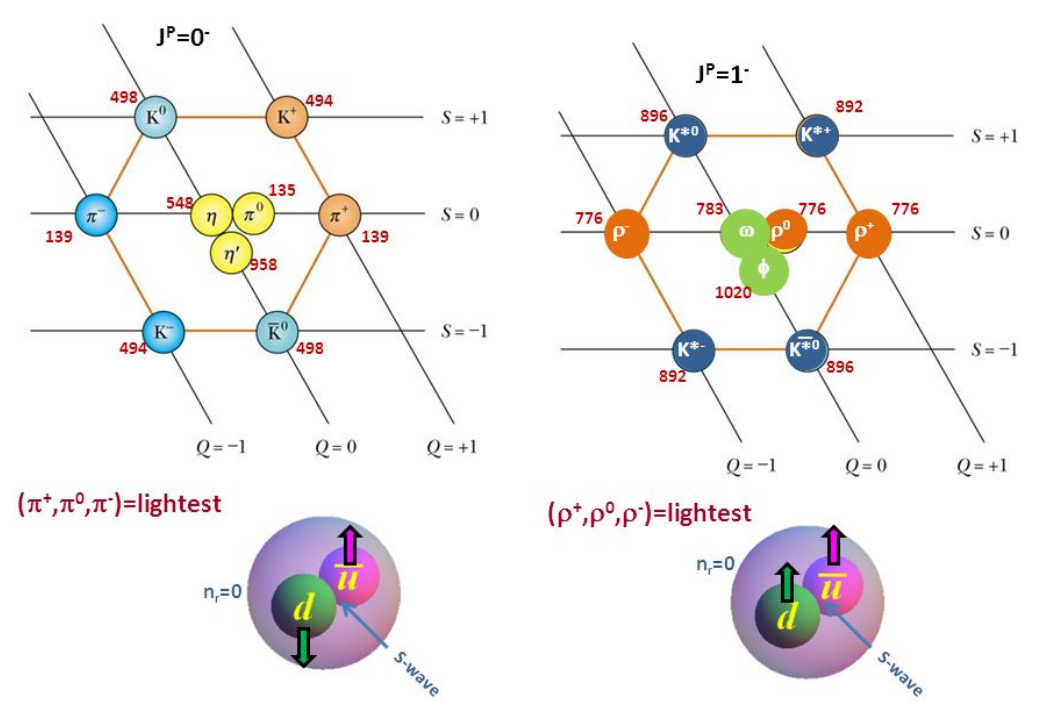
\includegraphics[width=250pt]{fig9_09}
\end{figure}

Anche in questi grafici gli assi indicano la carica e la stranezza.

\paragraph{$\Delta^{++}$ e $\Omega^-$: il numero di colore}
I quark sono fermioni per cui devono soddisfare il principio di esclusione di Pauli, che afferma che due particelle non possono stare nello stesso stato.
Un altro modo per dirlo è dire che la funzione d'onda complessiva che descrive un fermione deve essere antisimmetrica ovvero deve cambiare segno per inversione.
Per cui anche la funzione d'onda della $\Delta^{++}$ deve essere antisimmetrica, ma questo presenta delle difficoltà infatti questa particella ha spin totale $J=3/2$ e momento angolare nullo $L=0$, una particella però con $L=0$ ha una forma d'onda spazialmente simmetrica.
La funzione d'onda di questa particella è costituita come abbiamo visto da tre quark dello stesso tipo con lo stesso spin
\begin{equation}
|\Delta^{++}>=|u\uparrow u\uparrow u\uparrow>
\end{equation}
siccome hanno tutti e tre lo spin up anche la funzione d'onda di spin deve essere simmetrica.
Essendo costituita solo da quark di tipo up vuol dire che la funzione d'onda deve essere anche simmetrica per lo scambio di quark.
In questa forma quindi questa funzione d'onda non può essere antisimmetrica, abbiamo infatti tre quark che hanno praticamente gli stessi numeri quantici che danno una funzione simmetrica dal punto di vista spaziale, come funzione d'onda degli spin e anche dal punto di vista del flavour (scambio di quark).
Sembrerebbe dunque una violazione del principio di esclusione di Pauli.

Per risolvere la questione è stato introdotto un altro numero quantico, il numero di colore.
I quark possiedono quindi una proprietà ulteriore ossia il colore che esprime la dinamica tra i quark, come interagiscono tra di loro.
I colori possono essere tre: rosso $r$, verde $g$ e blu $b$.
Questi tre valori corrispondono a delle cariche dell'interazione forte che ne definiscono la dinamica.
Esistono poi anche dei valori corrispondenti per gli antiquark: antirosso $\bar{r}$, antiverde $\bar{g}$ e antiblu $\bar{b}$.

La carica di colore è ciò che da luogo ai gluoni e la sua rappresentazione è la stessa dei quark $u, d, s$ ossia con la creazione di un ottetto e un singoletto.
\begin{equation}
3 \otimes 3= 8 \oplus 1
\end{equation}
Le possibili combinazioni di $r, g, b$ sono quindi nove.
La forza forte quindi è molto più articolata della forza elettromagnetica, che per esempio si scambia solo tramite un  fotone per cui con uno stato unico di singoletto; si ha infatti che i quark interagiscono tramite colore e gli antiquark tramite anticolore.

Si chiama carica di colore perché la logica di combinazione per definire gli stati stabili rende gli adroni degli oggetti neutri rispetto al colore, che quindi a livello generale l'interazione forte non è poi così diversa dall'interazione elettromagnetica, considerando però un atomo.
Nel caso di colore perché un adrone esista bisogna fare in modo che la somma delle tre cariche di colore sia nulla.
La rappresentazione sfrutta solitamente uno schema a frecce.
\begin{figure}
\centering
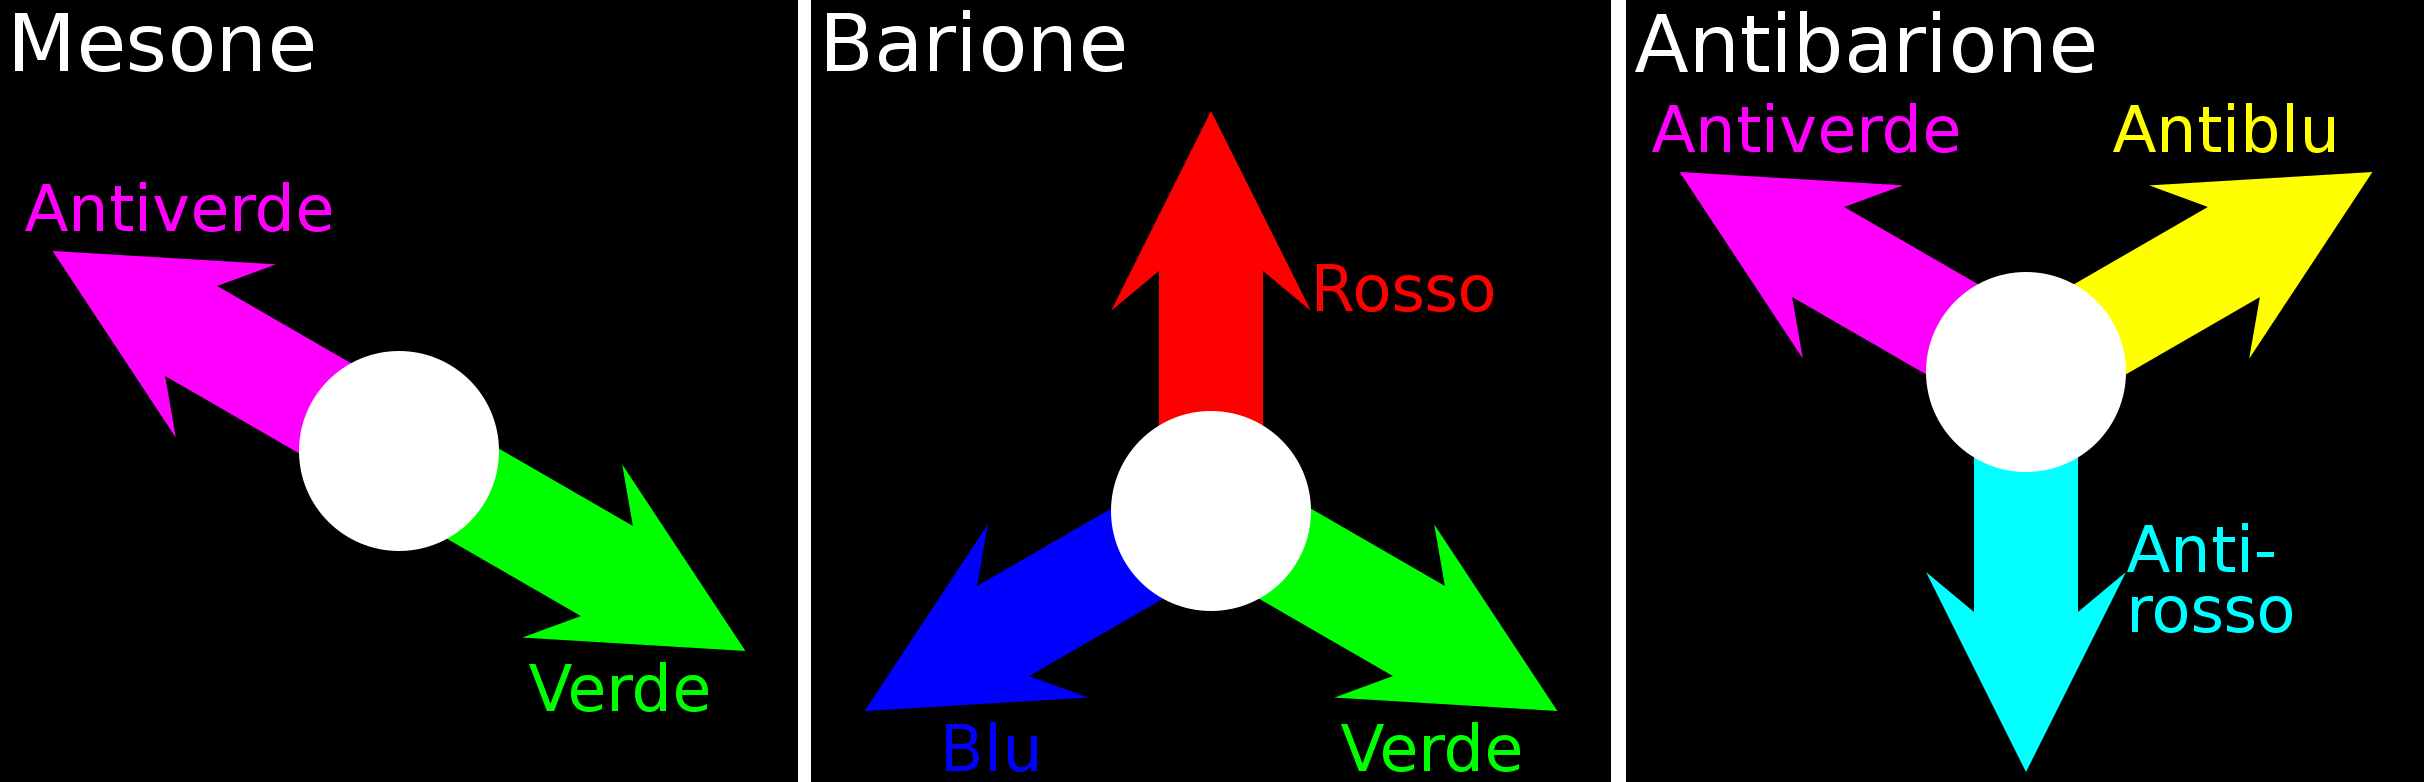
\includegraphics[width=200pt]{fig9_10}
\end{figure}

\paragraph{Cromo-dinamica quantistica}
La teoria che spiega e studia l'interazione di colore si chiama \emph{Cromo-dinamica quantistica (QCD)} ed è una di quelle teorie di campo che costituiscono il modello standard.
Anche in questo caso la simmetria è classificata nelle simmetrie di $SU(3)$ che è semplicemente un modo elegante per esprimere che la carica di colore totale debba essere sempre nulla.
Il motivo per cui non è mai possibile vedere un quark da solo è che un quark separato non avrebbe carica di colore nulla.
Per lo stesso motivo non esistono combinazioni del tipo $qq\bar{q}$.
Ovviamente questa trattazione serve a capirne la logica generale, il formalismo della forza forte è invece molto più complesso.

Una delle conseguenze di questo comportamento è la dipendenza della forza forte dal momento trasferito $Q^2$.
Se si rappresenta la costante di accoppiamento forte $\alpha_S$, che è la costante che esprime l'intensità della forza forte (è l'analogo della costante di struttura fine per la forza elettromagnetica), in funzione del momento trasferito si ottiene un andamento straordinario.
\begin{figure}
\centering
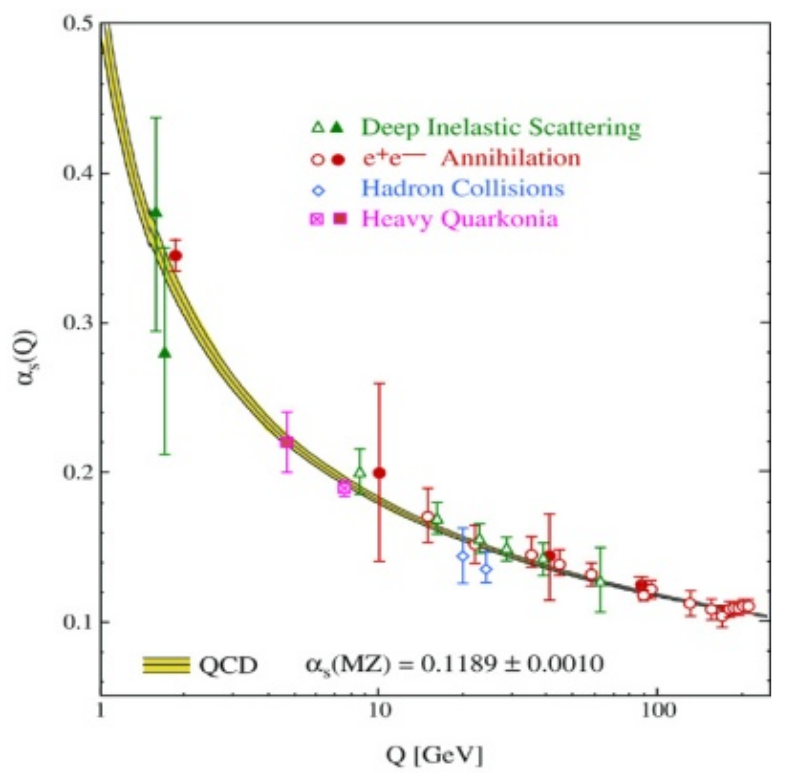
\includegraphics[width=180pt]{fig9_11}
\end{figure}

\'E inaspettato questo andamento in quanto con l'aumentare del momento trasferito ci si avvicina alle particelle, per cui ci si aspetterebbe che pure la carica aumentasse; in realtà la forza forte ha una logica totalmente opposta ovvero più ci si avvicina alla carica e più la sua intensità diminuisce.
Il fatto che se $r\to 0$ allora anche $\alpha_S$ tende a diminuire è chiamato \emph{libertà asintotica}; questo vuol dire che più due quark sono vicini e meno è la forza tra di loro.
Il fatto che se invece $r\to \infty$ allora $\alpha_S$ aumenta è chiamato \emph{confinamento} (questo rafforza ancora l'impossibilità di vedere i quark separati).

Per spiegare questo comportamento e la differenza che c'è con la costante elettromagnetica (che aumenta più ci si avvicina), bisogna considerare l'\emph{effetto di screening}.
Questo è comune sia all'interazione elettromagnetica che alla QCD.
Supponiamo di avere una carica di qualsiasi tipo (per l'esempio sfrutteremo una carica negativa).
\begin{figure}[h]
\centering
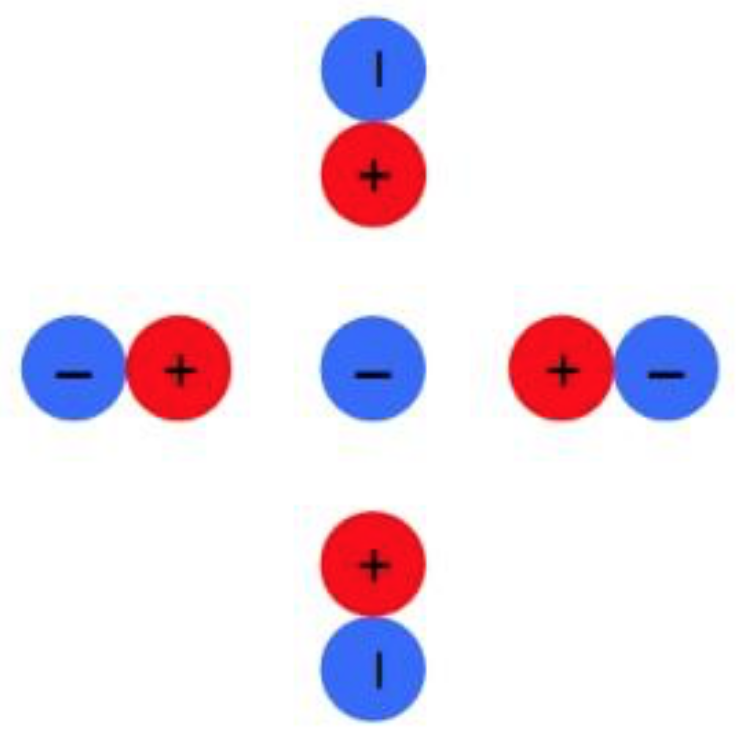
\includegraphics[width=180pt]{fig9_12}
\caption{Effetto di screening di una carica negativa}
\end{figure}

Una particella per far sentire la sua presenza emetterà un fotone virtuale che può decadere a sua volta in una coppia di particelle ci carica opposta (elettrone positrone), quello che succede è che se vedo la mia particella da lontano la carica interna risulta schermata da un effetto di polarizzazione del vuoto.
In termini di diagrammi di Feynman quello che succede è che il fotone si divide in due cariche prima di essere riassorbito nel vuoto, questo è un effetto reale e misurabile infatti non bisogna considerare il vuoto come il nulla ma piuttosto come una "ribollire" di energie, se infatti prendiamo una qualsiasi energia e la riemettiamo in un tempo adeguato non violiamo nessuna legge di conservazione energetica.
Effettivamente se ci avviciniamo ad una particella la carica di interazione elementare aumenta e questo è valido sia per l'elettromagnetismo che per la QCD.
La cromo-dinamica quantistica però è molto più complessa dell'elettromagnetismo infatti mentre un fotone non può avere interazione con altri fotoni il gluone, mediatore della forza forte, sì.
\begin{figure}[h]
\centering
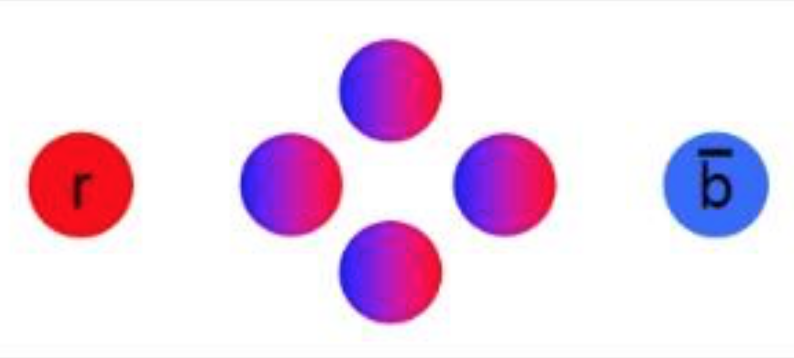
\includegraphics[width=180pt]{fig9_13}
\caption{Effetto di antiscreening della forza forte}
\end{figure}

Questo comporta il fatto che un gluone può dare luogo ad altri gluoni, supponendo quindi di avere un quark rosso e uno blu un gluone può essere blu e rosso e questa cosa comporta il fatto che la forza aumenta con l'aumento della distanza, provocando quello che è l'\emph{effetto di antiscreening}.

\paragraph{Potenziale di forza forte}
Prendiamo ora per esempio l'interazione di un elettrone con un protone, secondo la meccanica quantistica, ad un'energia adeguata, l'interazione avviene tra un fotone virtuale, emesso dall'elettrone, e un quark che compone il protone.
\begin{figure}[h]
\centering
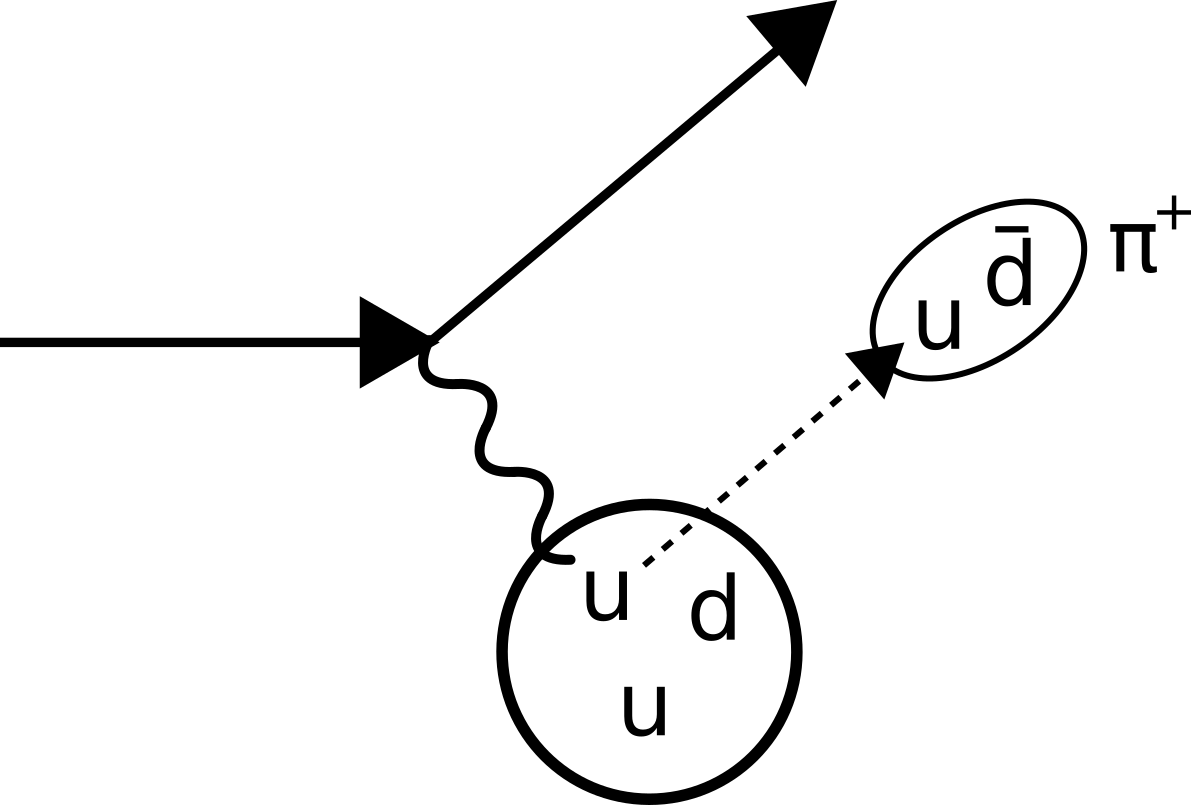
\includegraphics[width=200pt]{fig9_14}
\end{figure}

Il fatto che il quark si ecciti e tenda a dissociarsi dal protone provoca una forza forte dovuta all'allontanamento, che però è così forte da richiamare dal vuoto un'antiparticella che va a legarsi al quark portando alla generazione di un pione $\pi^+$.
Le linee di campo della forza forte si concentrano solamente nella regione di congiungimento tra le due particelle.

Quello che succede in poche parole è che l'allontanamento di due particelle provoca un aumento di energia potenziale tale da poter convertire l'energia generata in massa.
Anche se siamo passati ad una rappresentazione energetica tramite particelle virtuali è comunque possibile dare una rappresentazione del potenziale per la forza forte.
Facendo un grafico del potenziale in funzione della distanza tra le particelle quello che si può vedere è un grafico che ha un andamento come 
\begin{equation}
V_S=-\frac{4\alpha_S}{3r}+kr
\end{equation}
La prima parte della formula ricorda il potenziale coulombiano, quindi vediamo che a basse distanze i due potenziali hanno un andamento simile.
Se invece ci si allontana subentra il termine $kr$ che aumenta di molto il potenziale ricordando un po' quella che è la costante di una molla.
Il valore di questa costante è
\begin{equation}
k=1\frac{GeV}{fm}
\end{equation}
Per una migliore comprensione di cosa vuol dire questo valore scriviamo la formula della forza generata da questo potenziale
\begin{equation}
F=-\frac{dV}{dr}=+\frac{4}{3}\frac{\alpha_S}{r^2}+k
\end{equation}
Se $r$ è grande possiamo trascurare il primo termine ottenendo una forza pari a
\begin{equation}
F=k=1\frac{GeV}{fm}=\frac{1,6\times10^{-10}}{10^{-15}}N=1,6\times10^5N
\end{equation}
Che è la forza associabile a una massa di $16000kg$, e questa è la forza che si genera cercando di separare due quark!

\paragraph{Violazione dell'invarianza di scala}
Un'evidenza sperimentale dell'esistenza dell'esistenza dell'interazione tra i quark è quella che si chiama violazione dell'invarianza di scala nel \emph{deep inelastic scattering}.
Una delle risultanze sperimentali dell'evidenza dei quark era che i quark erano particelle puntiformi indipendentemente dalla lunghezza d'onda del fotone virtuale, quindi ricordando la funzione $F_2$, questa era dipendente solamente da $x$. 
Questa è ciò che viene chiamata invarianza di scala, siccome queste particelle non dipendono dalla lunghezza d'onda della sonda possono essere considerati puntiformi.
In realtà continuando a sperimentare si è visto che una leggera dipendenza $Q^2$ c'è.
Nei grafici sottostanti è mostrato questo effetto di dipendenza chiamata \emph{violazione dell'invarianza di scala}.
\begin{figure}
\centering
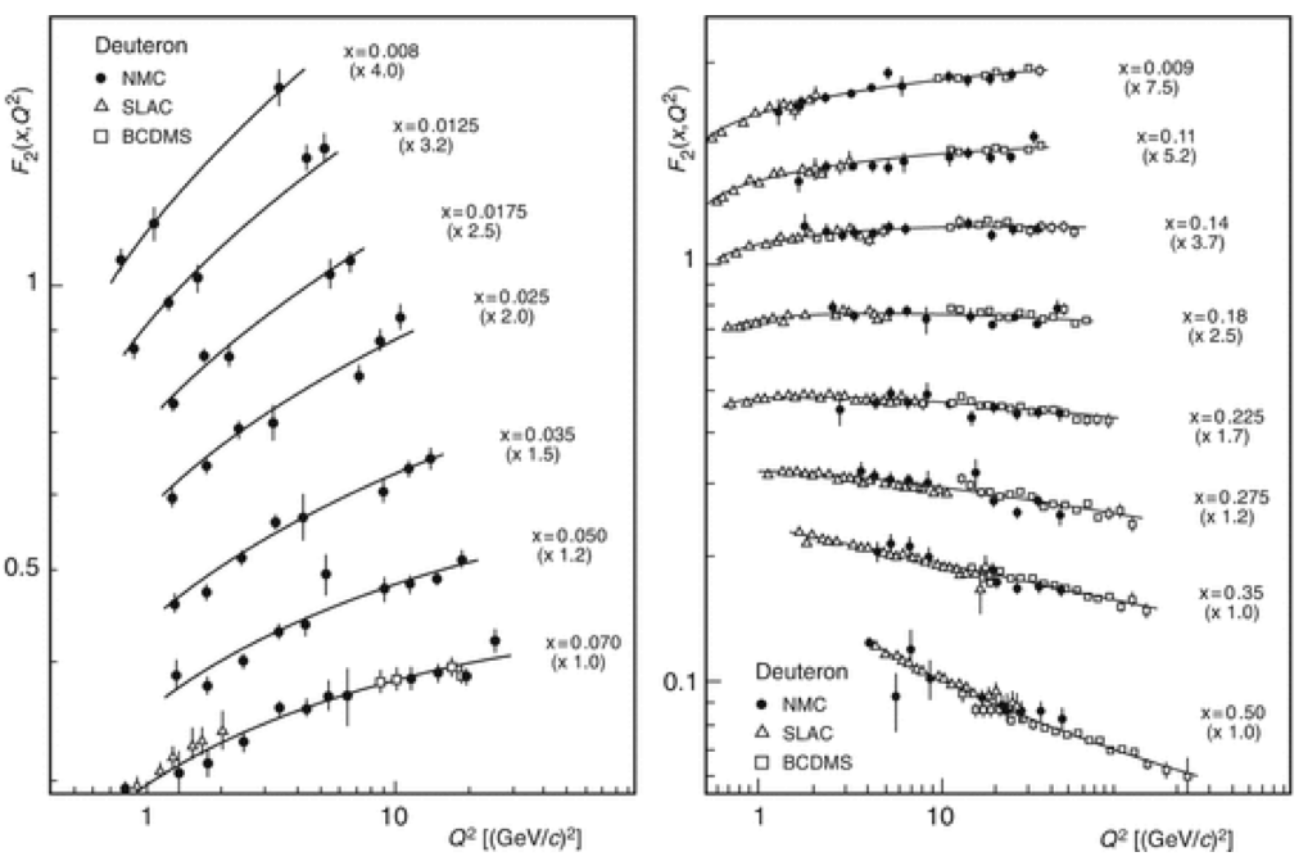
\includegraphics[width=200pt]{fig9_15}
\end{figure}

Il grafico a destra mostra la dipendenza ad alti x mentre a sinistra a bassi x, si sta parlando della \emph{x di Bjorken} quindi si sta parlando della frazione di momento portata dal partone analizzato.
Quello che si vede è che nei partoni che portano più alte frazioni di energia (grafico a destra) all'aumentare di $Q^2$ la \emph{x di Bjorken} diminuisce, il che vuol dire che se andiamo ad ispezionare il nucleo con lunghezze d'onda sempre minori è molto meno probabile che una grande parte della quantità di moto del protone sia portata da un unica particella.
Al contrario nel grafico a sinistra si ha che all'aumentare di $Q^2$ la frazione di partoni che portano una frazione più piccola di quantità di moto aumenta.
Questo vuol dire semplicemente che andiamo ad analizzare strutture sempre più piccole e allora è molto più probabile che i quark emettano muoni e che dunque la frazione di quantità di moto sia portata da un numero di particelle sempre maggiore.
Ad un $X$ basso aumenta il numero di particelle che si distribuiscono tra di loro la quantità di moto del protone, il modo con cui avviene questa distribuzione è l'interazione di quark che provoca l'emissione di gluoni che decadono portando all'emissione di altre particelle.
Questa in pratica è un'evidenza sperimentale dell'esistenza dei gluoni, questi infatti possono essere visti solo indirettamente in quanto non portano carica elettrica e quindi risultano invisibili altrimenti.
Possiamo quindi intuire che se $x$ aumenta o diminuisce il numero di particelle varia.

%nuova sezione-------------------------------------------------------
\subsection{Interazione debole}
L'interazione si chiama debole perché si manifesta in modo meno intenso della forza elettromagnetica e della forza forte.
Questo per esempio si può esprimere nella sezione d'urto.
Mentre nel caso della sezione d'urto della forza forte tra due protoni si ha un valore di
\begin{equation}
\sigma_{forte}(E>10GeV)\sim 50mb
\end{equation}
e nel caso della forza elettromagnetica si ha una sezione d'urto che può virtualmente essere considerata infinita (interazione a range infinito) ma che anche andando a vedere fino a quando ci sono effetti elettromagnetici ravvisabili ha un valore di 
\begin{equation}
\sigma_{el-mag}\sim 10mb
\end{equation}
la sezione d'urto di forza debole, è molto più piccola; prendendo per esempio un neutrino di energia $1MeV$, la sezione d'urto avrà un valore di 
\begin{equation}
\sigma_{debole}\sim 10^{-44}cm^2\sim 10^{-20}b
\end{equation}
Un altro parametro di "debolezza" di questa forza è la vita media delle particelle che decadono per interazione debole.
Uno stato che decade per interazione forte ha vita media pari a
\begin{equation}
\tau_{forte}\leq 10^{-20}s
\end{equation}
uno stato che decade per interazione elettromagnetica
\begin{equation}
10^{-12}s\leq \tau_{el-mag}\leq 10^{-20}s
\end{equation}
invece un decadimento di uno stato per interazione debole ha un tempo 
\begin{equation}
\tau_{debole} \geq 10^{-12}s
\end{equation}

Si è visto poi che la forza debole non è da considerarsi debole a causa della stessa interazione, infatti nell'interpretazione delle moderne teorie quantistiche di campo i bosoni vettori della forza debole sono stati visti essere estremamente massivi ed è questo che porta ad un "indebolimento" della forza; questo può essere portato all'estremo tanto che c'è una teoria che va ad unificare forza debole ed elettromagnetismo.

\paragraph{Universalità dell'interazione debole}
Una delle peculiarità dell'interazione debole è quella che si chiama \emph{universalità}.
L'interazione debole può avvenire in varie modalità diverse:

\begin{itemize}
\item \emph{Processi leptonici}; sono i processi che coinvolgono solamente leptoni.
Per esempio si è visto che ci sono due "cugini" pesanti dell'elettrone, il muone $\mu^-$ e il leptone $\tau$.
Il muone essendo più pesante dell'elettrone decade (con una vita media di $2\mu s$)
\begin{equation}
\mu^-\to e^-+\bar{\nu_e}+\nu_\mu
\end{equation}
Questa è una reazione che rispetta tutte le leggi di conservazione infatti è conservato anche il numero leptonico.
Inoltre la reazione, che Fermi considerava di contatto, si è visto che è in realtà mediata da un bosone vettore $W^-$ che decade nell'elettrone e nell'antineutrino elettronico.
\begin{figure}[h]
\centering
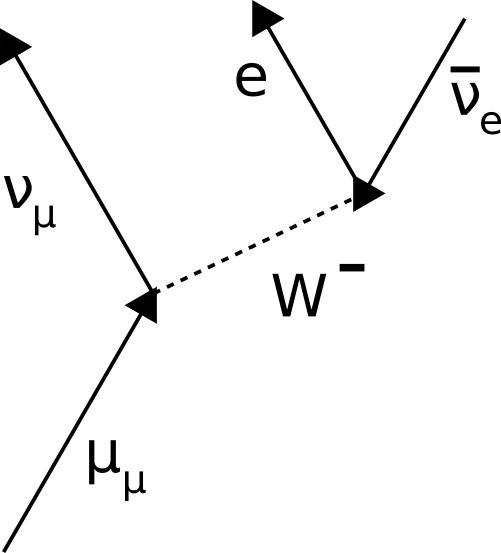
\includegraphics[width=150pt]{fig9_17}
\caption{Decadimento del muone}
\end{figure}

\item \emph{Processi semi-leptonici} che vanno a coinvolgere sia quark che leptoni.
Un esempio può essere il decadimento di un neutrone in un protone, che di base ha una dinamica del tutto simile al decadimento del muone ma con il coinvolgimento di due adroni.
Il processo può poi essere rivisto considerando l'interazione come un decadimento di un singolo quark all'interno del neutrone.
\begin{figure}[h]
\centering
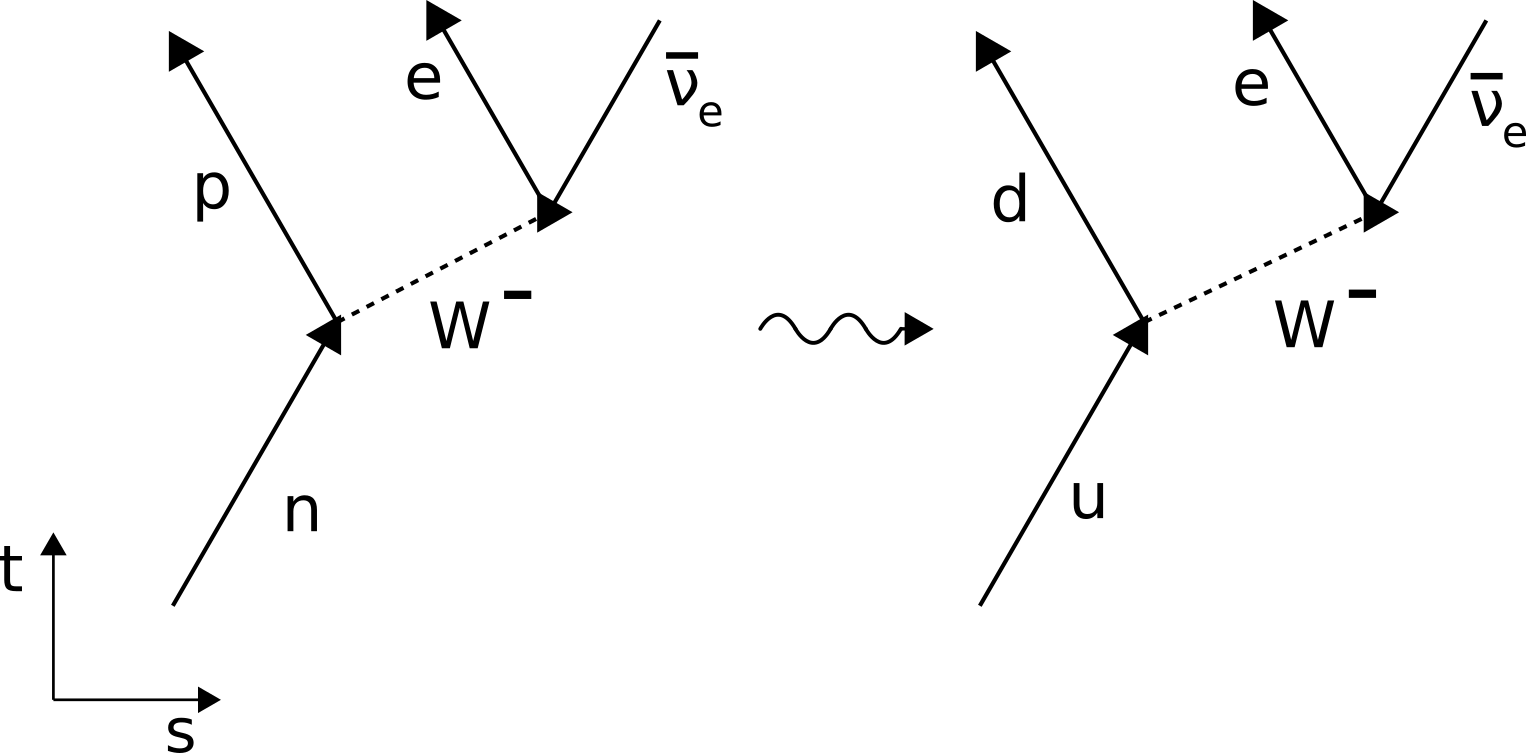
\includegraphics[width=300pt]{fig9_16}
\caption{Decadimento del neutrone}
\end{figure}
Un altro processo semi-leptonico è il decadimento del pione negativo
\begin{equation}
\pi^-\to \mu_\nu+\bar{\nu_\nu}
\end{equation} 
Il diagramma di Feynman di questo fenomeno è simile a quelli già visti.
C'è un altro mesone che decade così è il caone $K^+$.

\item \emph{Processi non leptonici} che coinvolgono solamente quark.
Un processo di questo tipo è un decadimento secondario del caone $K^+$
\begin{equation}
K^+\to \pi^++\pi^0
\end{equation}
\end{itemize}

\paragraph{Matrice d'interazione}
I diagrammi di Feynman non sono solo molto utili per lo scopo divulgativo ma danno anche un grande aiuto per quel che riguarda la scrittura delle matrici di interazione.
Si prenda come esempio il decadimento del muone $mu^+$
\begin{figure}[h]
\centering
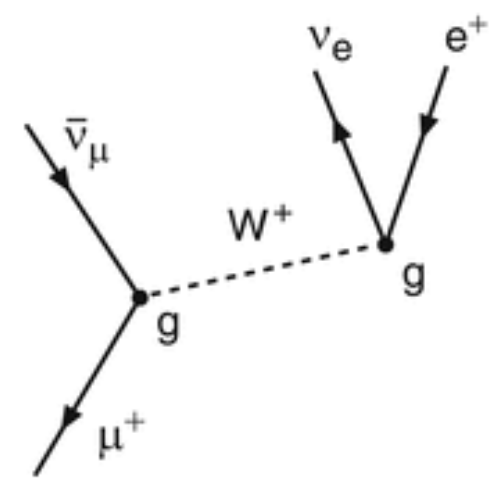
\includegraphics[width=150pt]{fig9_18}
\end{figure}

La matrice d'interazione tra lo stato iniziale e finale del processo sarà proporzionale a 
\begin{equation}
M_{i-f}\propto g\cdot \frac{1}{Q^2c^2+M^2_Wc^4}\cdot g
\end{equation}
dove $g$ è un fattore che tiene conto dell'intensità della reazione, considerato ai vertici dell'interazione; la frazione centrale è chiamata propagatore; $M^2_W$ è la massa della particella scambiata; $Q^2$ è il solito fattore di momento trasferito.

Se si considera ora l'approssimazione a bassi momenti trasferiti ($Q^2\to 0$) si ottiene
\begin{equation}
M_{i-f}\propto \frac{g^2}{M^2_Wc^4}
\end{equation}
$g^2$ è l'intensità, molto simile alla costante di struttura fine, infatti la costante di struttura debole si avvicina molto alla costante di interazione elettromagnetica ma il motivo per cui si vede la forza debole "debole" è a causa del termine $M^2_W$.

\paragraph{Matrice CKM: interazione debole tra i quark}
La matrice di Cabibbo-Kobayashi-Maskawa, è una matrice che descrive l'interazione debole tra i quark.
L'interazione debole è stata definita come universale, quello che si è però visto sperimentalmente è che la probabilità che un quark $up$ si trasformasse in un quark $down$ era molto diversa dalla probabilità che diventasse un quark $s$, questo genera delle problematiche legate al fatto che il tipo di interazione deve essere la stessa se si parla di un'interazione universale.
L'intuizione che risolse la questione fu teorizzata da Cabibbo e postula che gli autostati dell'interazione debole possano non essere gli stessi della massa, quindi che quando una particella è libera rimane se stessa, per esempio un quark $up$ rimane un quark $up$ con una certa massa ed un certo tipo di caratteristiche, quando però questa interagisce tramite interazione debole cambia la sua natura, in questo caso quindi un quark $up$ può decadere in una combinazione di quark $down$ e quark $s$.
Si ha quindi una rotazione dell'autostato della massa, il quark $up$ decade in una composizione data da
\begin{equation}
u\longrightarrow \cos\theta_C d+\sin\theta_C s
\end{equation}
dove $\theta_C$ è chiamato \emph{angolo di Cabibbo}.
Volendo quindi rappresentare gli stati dell'interazione debole ciò che si ottiene è rappresentata in figura
\begin{figure}[h]
\centering
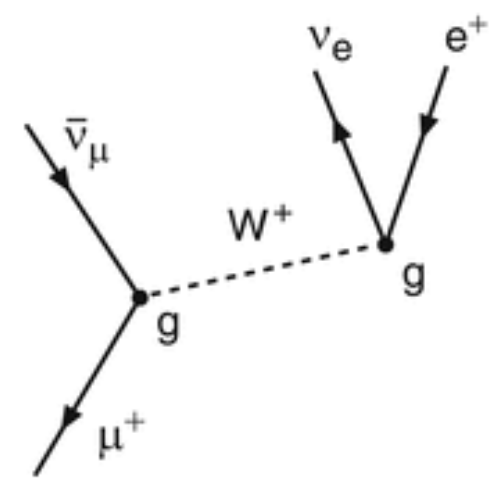
\includegraphics[width=180pt]{fig9_18}
\caption{Autostati ruotati dell'interazione debole}
\end{figure}
In altre parole non è detto che ciò che interagisce tramite questa forza corrisponda esattamente alla massa.
Si prendano ora le matrici di interazione, già viste in precedenza
\begin{equation}
\begin{pmatrix}
u\\d
\end{pmatrix}
\hspace{0.5cm}
\begin{pmatrix}
e\\s
\end{pmatrix}
\hspace{0.5cm}
\begin{pmatrix}
t\\b
\end{pmatrix}
\end{equation}

La combinazione di quark che interagiscono debole viene data, in termini matriciali, dalla formula (dove per convenzione si ruotano sempre i quark con carica $-1/3$)
\begin{equation}
\begin{bmatrix}
d'\\s'
\end{bmatrix}
=\begin{bmatrix}
\cos\theta_C&\sin\theta_C\\
-\sin\theta_C&\cos\theta_C
\end{bmatrix}
\begin{bmatrix}
d\\s
\end{bmatrix}
\end{equation}


Con questo tipo di intervento si è salvata l'universalità dell'interazione debole, viene infatti spiegato il motivo per cui la probabilità, anche per piccoli angoli di Cabibbo, è più alta verso il quark $d$ rispetto al quark $s$
Anche se potrebbe sembrare un artificio matematico in realtà quest'applicazione è dimostrata e ha una validità anche nella realtà.
Per considerare la casistica generale introduciamo la \emph{matrice CKB} che determina le probabilità di decadimento da e verso tutti i quark
\begin{equation}
\begin{bmatrix}
d'\\s'\\b'
\end{bmatrix}
=\begin{bmatrix}
v_{ud}&v_{us}&v_{ub}\\
v_{cd}&v_{cs}&v_{cb}\\
v_{td}&v_{ts}&v_{tb}
\end{bmatrix}
\begin{bmatrix}
d\\s\\b
\end{bmatrix}
\end{equation}
dove $d, s, b$ indica i quark $down, strange, bottom$, mentre ogni $v_{ij}$ indica la probabilità di decadimento da un quark $i$ verso un quark $j$ ($u, c, t$ indicano rispettivamente i quark $up, charm, top$).
 
Tutte queste probabilità sono state attualmente trovate sperimentalmente.
Quindi ogni quark interagisce con una combinazione lineare dei tre quark opposti.

\subsection{Violazioni di simmetria}
In natura esistono simmetrie continue ma anche simmetrie discrete.
Queste sono tre:
\begin{itemize}
\item \emph{Coniugazione di carica}, si indica con la lettera $C$ e sostituisce ad una particella la propria antiparticella, per esempio all'elettrone $e^-$ sostituisce il positrone $e^+$.
Ci sono anche particelle che sono la propri stessa antiparticella, per esempio il fotone, che non ha carica è esso stesso la sua antiparticella.

L'elettromagnetismo, la gravità e la forza forte sono simmetriche per $C$.
Un'operazione di simmetria è un cambiamento, una rotazione. 
In questo caso noi abbiamo una rotazione in uno spazio funzionale.
Un oggetto è simmetrico rispetto ad un'operazione di simmetria se dopo la rotazione risulta invariato.
Nel caso quindi delle forze elencate sopra si possono sostituire le particelle con le proprie antiparticelle e l'interazione non cambia, risultano quindi insensibili alle rotazioni di carica.

\item \emph{Parità} che significa inversione delle coordinate spaziali.
Vuol dire sostituire a 
\begin{equation}
\begin{split}
\vec{r}\to -\vec{r}\\
\vec{p}\to -\vec{p}\\
\end{split}
\end{equation}
Se io inverto posizione o quantità di moto delle varie particelle ottengo esattamente l'inverso.

Ciò non avviene nel caso del momento angolare 
\begin{equation}
\vec{L}\to \vec{L}
\end{equation}
Quello però che si può vedere è che anche in questo caso l'elettromagnetismo, la gravità e la forza forte soddisfano alla condizione di simmetria.

\item \emph{Time reversal}, vuol dire sostituire al tempo l'inverso del tempo.
Anche in questo caso le tre forze maggiori sono insensibili alla variazione.
Se si inverte il tempo, le leggi che le regolano sono le stesse.
\end{itemize}

Soffermiamoci ora sulla simmetria di parità perché è importante nella comprensione della forza debole.
Date le coordinate $x, y, z$, si effettua quindi una sostituzione con le antitetiche.
\begin{equation}
P
\begin{pmatrix}
x\\y\\z
\end{pmatrix}
=
P
\begin{pmatrix}
-x\\-y\\-z
\end{pmatrix}
\end{equation}
La simmetria di Parità afferma quindi che nel caso di trasformazioni di questo tipo le leggi non devono cambiare.

In geometria si sono viste le trasformazioni per rotazione, in fuzione di queste gli oggetti possono essere:
\begin{itemize}
\item scalari
\item vettori
\end{itemize}
Uno scalare è invariante per la rotazione mentre il vettore cambia segno.
Con l'operazione di parità si introducono anche quantità
\begin{itemize}
\item pseudo scalari (anch'essi invarianti per rotazione)
\item vettori polari (per esempio la quantità di moto) si invertono per rotazione, possedendo quindi parità $P=-1$
\item vettori assiali, con parità $P=+1$, ma si comportano come vettori rispetto alla rotazione
\end{itemize}
\'E importante distinguere tra vettori assiali e vettori polari, infatti sono entrambi vettori ma per quanto riguarda l'inversione di parità i comportano in modo diverso.

Introduciamo quindi due casistiche.

I \emph{vettori e scalari normali} sono quelli che si comportano "normalmente" rispetto alla parità.

Un vettore normale applicando la parità subisce la trasformazione
\begin{equation}
\begin{split}
\vec{r}&\to -\vec{r}\\
\vec{p}=m\vec{\dot{r}}&\to  -m\vec{\dot{r}}=-\vec{p}
\end{split}
\end{equation}
Un vettore normale per parità inverte quindi le proprie coordinate.

Uno scalare normale invece non subisce variazioni rispetto alla parità.
Si consideri per esempio  la norma 
\begin{equation}
r=(\vec{r}\vec{r})^{\frac{1}{2}}\to [(-\vec{r})(-\vec{r})]^{\frac{1}{2}}=(\vec{r}\vec{r})^\frac{1}{2}=r
\end{equation}

I \emph{pseudo vettori e pseudo scalari} invece sono quelli che rispetto alla parità si comportano in modo anomalo.

Si consideri per esempio il vettore momento angolare
\begin{equation}
\vec{L}=\vec{r}\times \vec{p}\to (-\vec{r})\times (-\vec{p})=\vec{r}\times \vec{p}=\vec{L}
\end{equation}
In questo caso quindi il momento angolare che è un \emph{vettore assiale} è definito anche \emph{pseudo vettore} perché rispetto alla parità si comporta in modo diverso dai vettori.

\paragraph{Prova sperimentale della violazione di parità}
Prima dell'interazione debole si dava per scontato che tutte le leggi della fisica rispettassero la parità.
L'esperimento che rivoluzionò questa concezione fu teorizzato da due fisici cinesi e eseguito da Madame Wu.
Questo esperimento coinvolgeva l'elicità e si basava semplicemente sul prendere un nucleo di cobalto e orientare gli spin in un certo modo.

In pratica si prende questo nucleo che ha un certo spin, quindi un certo momento magnetico, e lo si pone all'interno di un campo magnetico, in questo modo si ottengono tutti gli spin orientati allo stesso modo.
Quello che si verificava è che prendendo un atomo di cobalto, orientato secondo il campo magnetico, con un momento magnetico, rotante lungo un piano conosciuto, questa effettuerà decadimento $\beta$; si è visto sperimentalmente che gli elettroni così generati venivano emessi principalmente nella direzione opposta allo spin del cobalto.
Questo era sufficiente per dire che l'interazione debole viola il principio di parità.

Per capire quello che succede si consideri uno specchio piano, questo ha la proprietà di invertire virtualmente la coordinata spaziale ortogonale ad esso.
Se si vede l'esperimento appena descritto all'interno di uno specchio ciò che si verifica è che lo specchio inverte solo la coordinata perpendicolare ad esso, per cui gli elettroni andranno in verso opposto, si ha però che il momento angolare magnetico rimane invariato.
Quello che però si vede nello specchio è solamente virtuale e quindi non esiste!
Questo basta a determinare la violazione della parità infatti se così non fosse non dovrebbe esserci una direzione privilegiata ma le particelle dovrebbero essere emesse isotropicamente.
\begin{figure}[h]
\centering
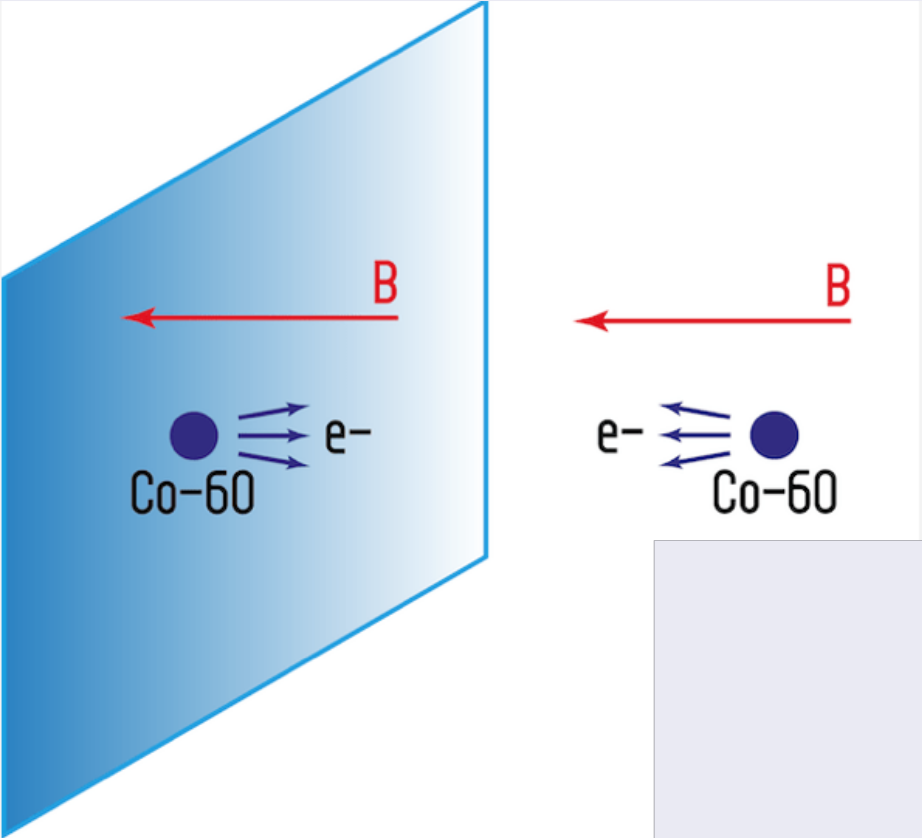
\includegraphics[width=180pt]{fig9_20}
\caption{Violazione di parità}
\end{figure}

\paragraph{Esperimento di Goldhaber}

I neutrini hanno una caratteristica importante per quanto riguarda la loro elicità.
Ricordo che quando abbiamo definito l'elicità abbiamo menzionato anche la chiralità.
Queste due grandezze pur rappresentando la stessa grandezza hanno una differenza sostanziale ovvero se una particella non si muove alla velocità della luce abbiamo visto che si può definire l'elicità, che avrà valore positivo o negativo in base al punto di osservazione, se però prendiamo in considerazione la particella alla velocità della luce l'elicità diventa chiralità e questa è un invariante caratteristica della particella.
Il concetto di base rimane comunque lo stesso.

L'esperimento di \emph{Goldhaber} ha avuto come scopo la misura dell'elicità del neutrino e sarà anche l'esperimento che ci aiuterà a capire come mai l'emissione del cobalto avvenga in una direzione preferenziale.
Il problema per misurare l'elicità del neutrino è il fatto che questo è una particella estremamente elusiva, il che comporta una difficoltà in una qualsiasi misura.
Bisogna quindi trovare un sistema diverso per effettuare la misura.
L'esperimento utilizzava la cattura elettronica su un nucleo di Europio $^{152}Eu$.
L'Europio presenta un momento angolare nullo nello stato utilizzato.
Questo inoltre faceva cattura elettronica, per cui il nucleo acquisiva un elettrone provocando il decadimento di un protone in un neutrone con l'emissione di un neutrino.
Il decadimento che avviene è del tipo
\begin{equation}
^{152}Eu+e^-\to ^{152}Sm^*+\nu +950keV
\end{equation}
Essendo poi il samario in un stato eccitato questo decade ulteriormente nello stato fondamentale con l'emissione di un fotone
\begin{equation}
^{152}Sm^*\to ^{152}Sm+\gamma+961keV
\end{equation}
L'unica diagnostica che si ha è l'emissione del raggio gamma, il concetto di base è dunque quello di riuscire a relazionare questi fotoni emessi con il neutrino.

Questo esperimento è piuttosto complesso e si divide in tre punti concettuali.
\begin{enumerate}
\item Correlazione tra l'elicità del fotone $\gamma$ emesso e del $\nu$.
Per fare ciò si sfrutterà la conservazione del momento angolare.
\item Correlazione tra la quantità di moto del $\gamma$ e del $\nu$.
Si sfrutteranno qui i concetti del rinculo del nucleo e dell'assorbimento risonante.
\item Misura dell'elicità del $\gamma$, tramite l'interazione con un bersaglio di ferro.
\end{enumerate}

Abbiamo visto sopra il processo di decadimento interessato, ciò che ora ci interessa è il momento angolare ottenuto dopo la cattura elettronica, partiamo infatti da un momento nullo.
L'elettrone assorbito porta con sé momento angolare $+1/2$ oppure $-1/2$, quindi all'atto della cattura elettronica ci ritroveremo con momento angolare corrispondente a quello elettronico.
Si ha poi che il samario si trova in uno stato eccitato con momento angolare $\pm 1$, questo comporta al fatto che il neutrino dovrà avere spin $-1/2$ nel caso di spin $+1$ del samario e $+1/2$ nel caso di spin $-1$ del samario.
Se si considera ora il decadimento allo stato fondamentale del samario, questo tornerà ad avere spin $0$ quindi per conservazione del momento angolare lo spin del samario sarà portato dal fotone emesso.
Si ottiene così una correlazione diretta tra lo spin del neutrino e lo spine del fotone.
\'E stato trovato il punto $1$.
 
Passando al punto $2$ si consideri il sistema di rivelazione.
Il materiale usato come rivelatore è samario formato da nuclei dello stesso tipo del samario di decadimento.
Dal processo di decadimento $\gamma$ è noto che per avere riassorbimento del fotone con un decadimento a due corpi è necessario
che le due emissioni abbiano stessa direzione e verso opposto.
Sarà quindi possibile rivelare solamente i fotoni che avranno neutrini emessi in direzione opposta. 
Ho così congelato l'elicità del neutrino perché misurando il fotone misuro la proiezione della quantità di moto sullo spin, perché solo il fotone posto back to back può esseere riassorbito da un altro atomo di samario.
Il gamma ha un'energia tale da portare il nucleo fuori risonanza.
\'E stato trovato anche il punto $2$.

Resta ora da capire solamente come misurare l'elicità del fotone.
Per fare ciò si fa interagire il fotone con un nucleo di ferro, questo interagisce con una sezione d'urto che è maggiore se gli spin di particella e nucleo sono perpendicolari rispetto a paralleli.
\begin{equation}
\frac{d\sigma}{d\Omega}(\uparrow\downarrow)>\frac{d\sigma}{d\Omega}(\uparrow\uparrow)
\end{equation}
Quindi applicando un campo magnetico si orientano gli spin del ferro in un certo modo e si avrà un certo tipo di assorbimento, poi è possibile invertire il campo generando quindi un inversione dello spin del ferro, vedendo quindi con che spin i fotoni vengono assorbiti maggiormente posso capire qual'è l'elicità dei fotoni emessi e di conseguenza anche di neutrini.

La scoperta fatta fu che l'elicità del fotone era pari a 
\[
H(\gamma)=-1,0\pm 0,3
\]
Il che vuol dire che i neutrini che interagiscono per interazione debole sono sinistrorsi ($LH$ left-handed), e questo è un concetto che viola chiaramente la parità.
A volte questo tipo di affermazione viene esagerata infatti ciò non deve indurre a pensare che tutti i neutrini siano sinistrorsi, ma piuttosto che i neutrini che interagiscono per interazione debole lo siano (lo stesso discorso può essere fatto per gli antineutrini che non sono necessariamente tutti destrorsi).

Più in generale si può dire che l'interazione debole interagisce solo con la parte sinistrorsa delle particelle e destra delle antiparticelle, per esempio anche l'interazione debole tra quark agisce allo stesso modo pur essendo particelle che avendo massa possiedono parte sia destrorsa che sinistrorsa.
Questo genera un problema infatti quelli che riusciamo a rivelare sono esclusivamente neutrini sinistrorsi e antineutrini destrorsi in quanto queste particelle interagiscono esclusivamente debolmente.
Per questo motivo i neutrini destrorsi, se esistono, vengono chiamati sterili.
L'interazione debole per conseguenza diretta viola anche la simmetria di carica perché sostituendo un neutrino sinistrorso con la sua antiparticella, questa dovrebbe essere un antineutrino sinistrorso ma l'interazione debole interagisce esclusivamente con i neutrini destrorsi.
La violazione di questo tipo viene detta violazione massimale in quanto non vi è alcuna interazione con queste particelle.

\paragraph{Simmetria combinata di carica $C$ e parità $P$}
Prendendo un neutrino sinistrorso, facendo la simmetria di parità si dovrebbe ottenere un neutrino destrorso che però non interagisce debolmente.
\begin{equation}
\nu_L\longrightarrow \nu_R
\end{equation}
Facendo poi la simmetria di carica ciò che bisognerebbe ottenere è
\begin{equation}
\nu_L\longrightarrow \bar{\nu_L}
\end{equation}
che anche questa volta non può interagire.

Applicando però entrambe le simmetrie si ottiene 
\begin{equation}
\nu_L\longrightarrow \bar{\nu_R}
\end{equation}
che è l'altra particella che interagisce per interazione debole.
Si ha quindi che l'interazione debole viola massimamente le simmetrie di carica e di parità però conserva la combinazione delle due simmetrie.

\'E stato effettuato un esperimento sui Kaoni $K$ in cui si è testata questa proprietà combinata.
Queste particelle hanno una componente strange e inoltre $K_0$ è una particella che è l'antiparticella di sé stessa.
Si sono studiato i decadimenti di questa particella, in particolare c'è una particella che si chiama $K_{short}$ e una che si chiama $K_{long}$.
Se la simmetria di $CP$ fosse stata mantenuta queste particelle avrebbero dovuto avere valore di $CP$ pari a $+1$, in realtà si è visto che in alcuni tipi di decadimenti questa simmetria è violata, quindi l'interazione debole viola anche la simmetria combinata di $CP$.

Si ha inoltre che se la simmetria di $CP$ è violata ma la simmetria di $CPT$ no, ci sarà per forza anche una violazione dell'inversione temporale $T$.
Ci sono quindi molti studi che si stanno concentrando su questo tipo di violazione combinata.
Questo interesse è dovuto anche al fatto che manca ancora una spiegazione alla disparità tra materia e antimateria, o meglio si hanno delle spiegazioni ma insufficienti ad evidenziare una disparità così grande, ci sono 8 ordini di grandezza inspiegati.